\documentclass{article}

\usepackage[utf8]{inputenc}
\usepackage{amsmath}
\usepackage{amsfonts}
\usepackage{amssymb}
\usepackage{graphicx}
\usepackage[table,xcdraw]{xcolor}
\usepackage[hidelinks]{hyperref}
\usepackage{fontawesome5}
\usepackage{longtable}


\graphicspath{ {./images/} }

\renewcommand{\contentsname}{Indice}

\makeatletter
\newcommand*{\rom}[1]{\expandafter\@slowromancap\romannumeral #1@}
\makeatother

\usepackage[a4paper,top=2cm,bottom=2cm,left=2cm,right=2cm]{geometry}


\title{\textbf{\Huge Sviluppo Applicazione}}
\author{Edoardo Ghirardello, Giulio Cappelli, Elia Casotti \\ \\ Gruppo T42}
\date{2022}

\let\origthesubsection\thesubsection

\begin{document}

\maketitle

\clearpage
\tableofcontents
\clearpage

\section{Scopo del documento}
\begin{description}
    \item[] Nel documento corrente vengono riportate ulteriori e definitive informazioni riguardo allo sviluppo dell'applicazione Fen Festa.
        \\ Nello specifico, presenta tutti gli artefatti necessari per il login, la ricerca e la creazione degli eventi dell'applicazione. In partenza viene analizzato lo User-flow legato ad un utente registrato dell'applicazione, dopodiché vengono analizzate le API (tramite l'API Model) per la creazione, modifica e login di un profilo, le strutture dati, la visualizzazione, creazione e modifica di un evento necessari a Fen Festa.
    \item[] Per ogni API che è stata utilizzata, vengono presentate descrizione delle funzionalità, documentazione e test utilizzati
    \item[] In ultima istanza vengono fornite informazioni del Git Repository e, infine, il deployment dell'applicazione.
\end{description}
\clearpage
\section{User-Flows}
\begin{description}
    \item[] In questa sezione vengono riportati gli “user-flows” dell'utente registrato (che quindi può anche essere organizzatore o admin) della nostra applicazione.
    \item[] In \hyperref[img:1]{Figura 1} viene mostrato lo user-flow relativo alle azioni disponibili dall'homepage dagli utenti: visualizzazione, partecipazione e aggiunta preferiti degli eventi; in aggiunta anche la creazione evento se l'utente ha i permessi da organizzatore.
    \item[] L'utente può visualizzare gli eventi tramite mappa o calendario e aggiungerli ai preferiti, in entrambi i casi, una volta avvenuta la visualizzazione di questi ultimi. Lo schema utilizza la notazione “Pausa” quando l'azione non è disponibile e la notazione “Arrivo” quando viene raggiunta l'ultima azione disponibile per quel ramo.
    \item[] Viene, inoltre, presentata una legenda che descrive i simboli utilizzati, sempre in \hyperref[img:1]{Figura 1}.
    \item[] \label{img:1} \begin{center}
            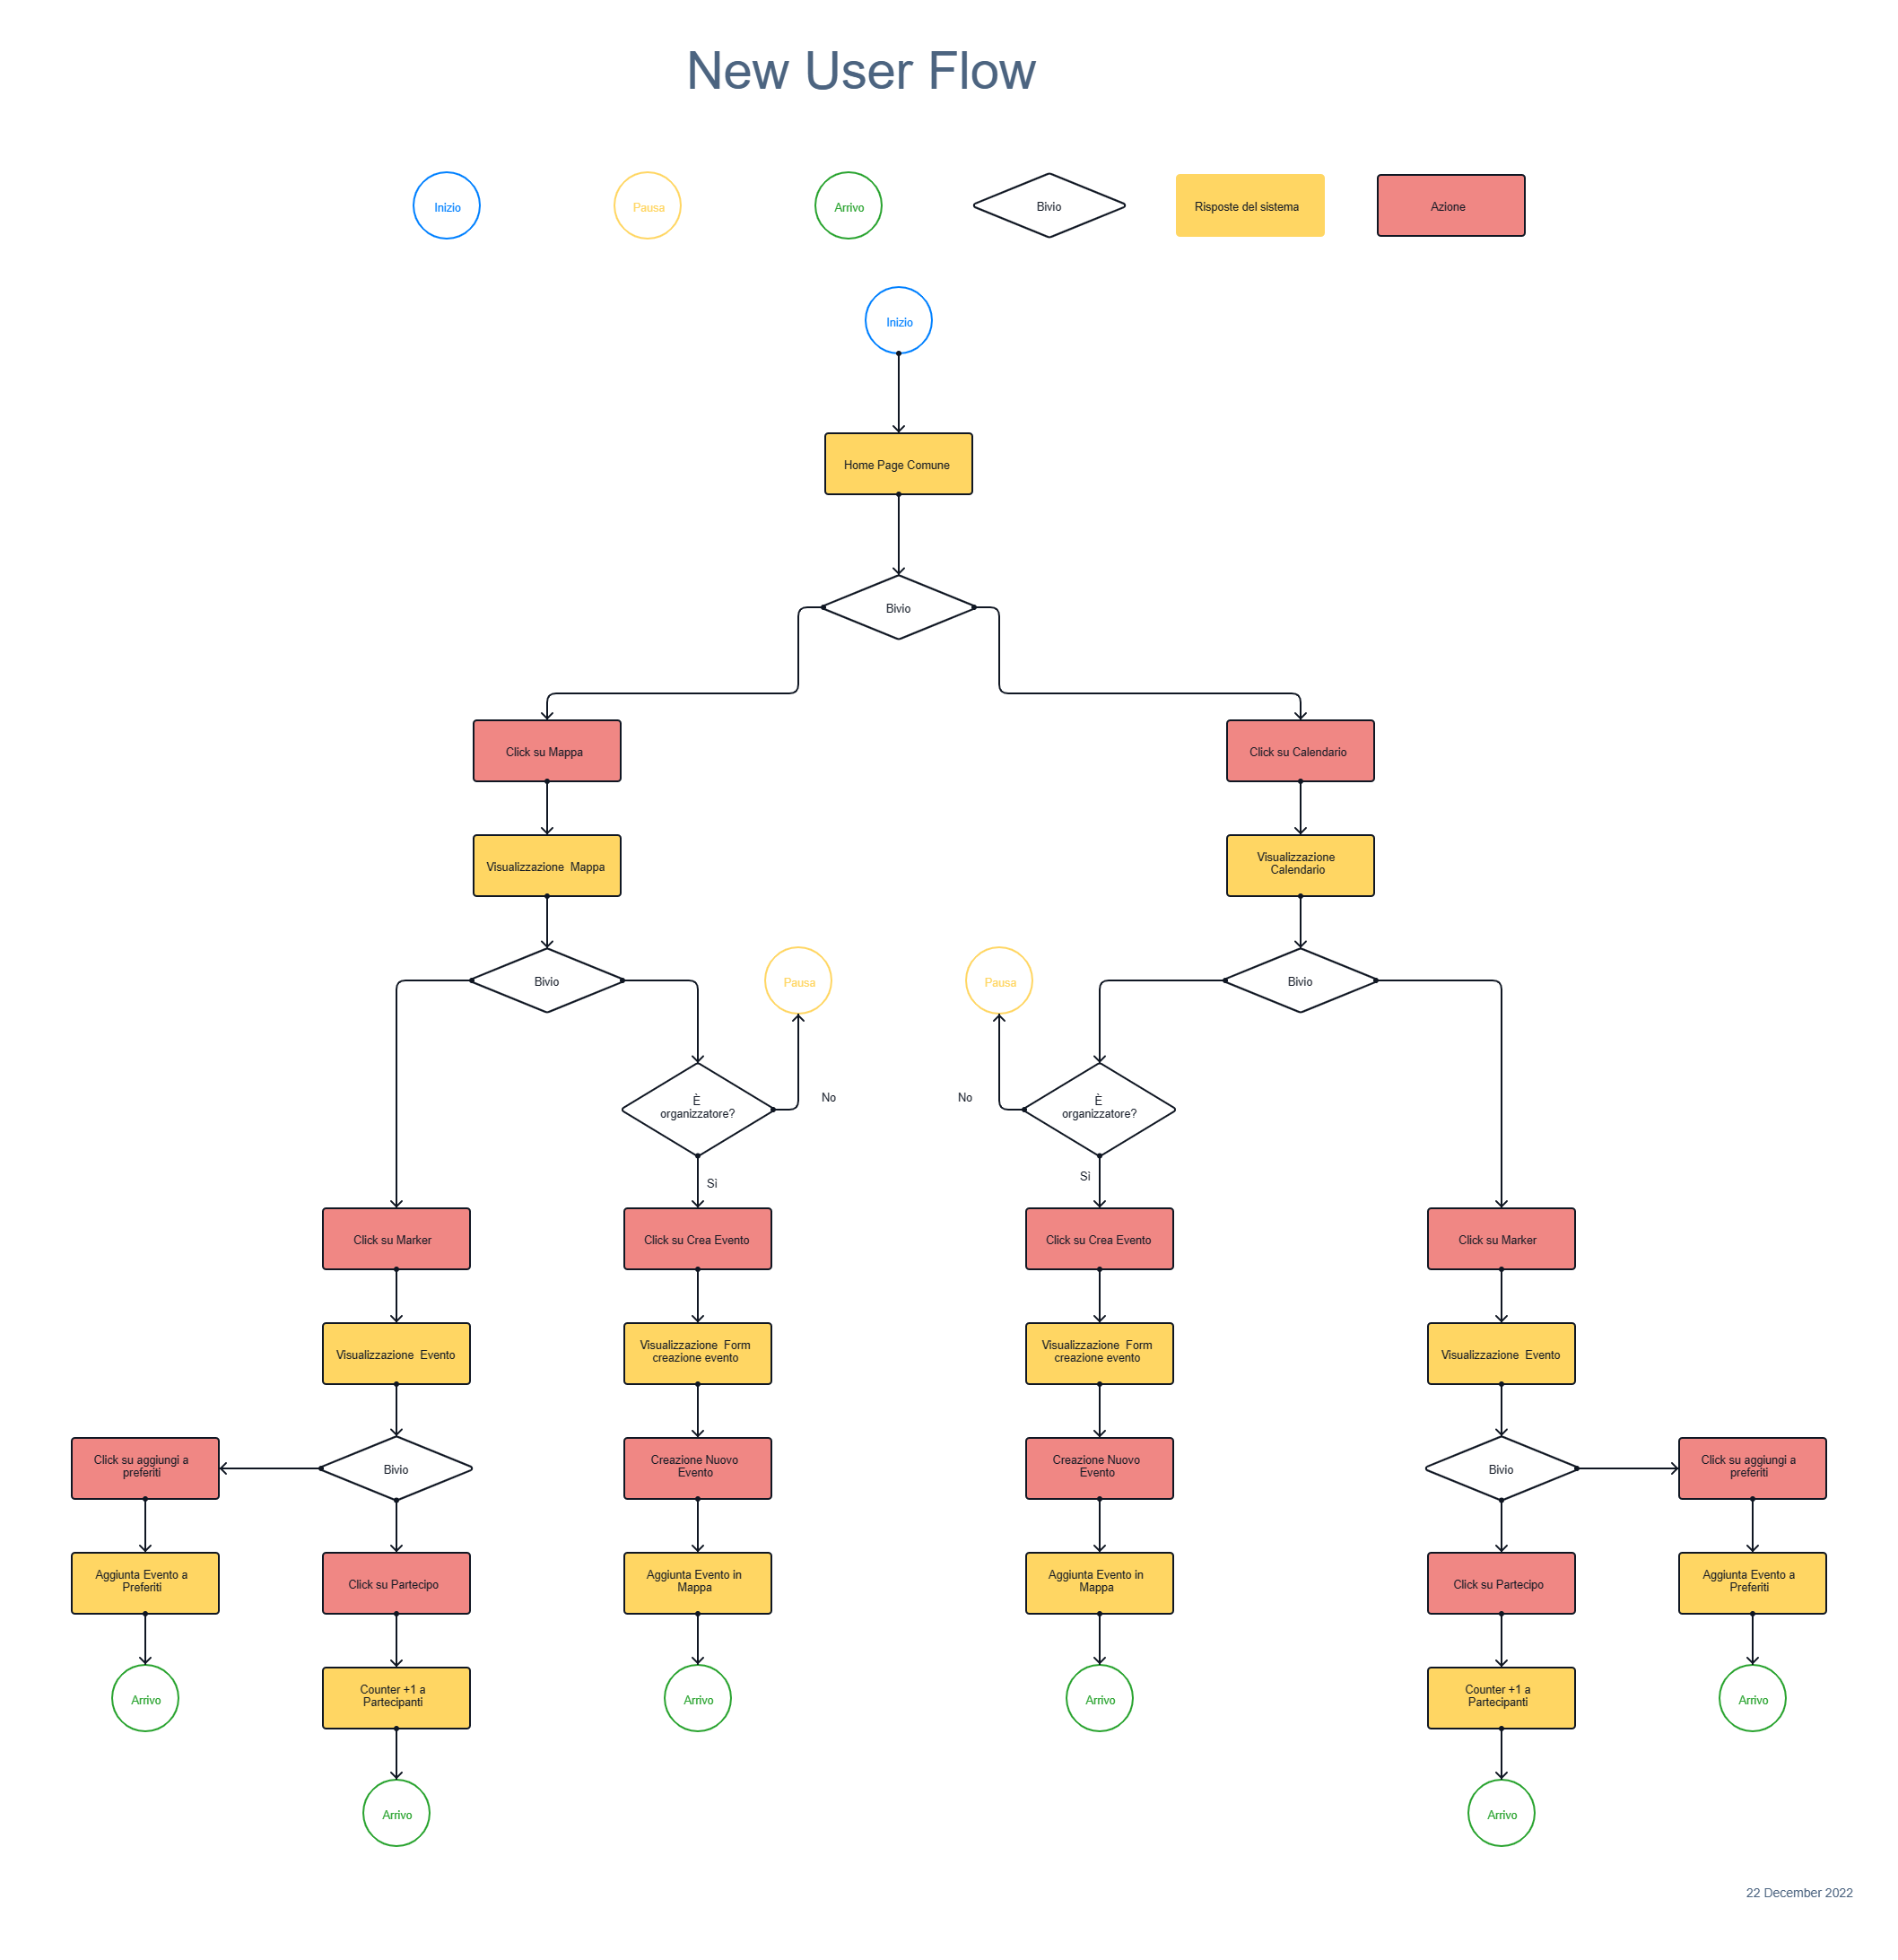
\includegraphics[scale=0.225]{User-Flow.png}
        \end{center}
\end{description}
\clearpage
\section{Application Implementation and Documentation}
\begin{description}
    \item[] Nei precedenti documenti sono stati identificati tutti i requisiti funzionali e non funzionali
        dell'applicazione. Nella sezione precedente son state descritte le features che servono ad un Utente nel
        suo flusso applicativo.
    \item[] Nella seguente sezione vengono analizzati i software e i tools di sviluppo di Fen Festa. L'applicazione è
        stata sviluppata utilizzando React (front-end) e Express (back-end). Per la gestione dei dati è stato utilizzato MongoDB.
\end{description}
\subsection{Project Structure}
\begin{description}
    \item[] Presentiamo in questa sezione la struttura del back-end, osservabile nell'immagine successiva \hyperref[img:2]{(Figura 2)}.
    \item[] \label{img:2} \begin{center}
            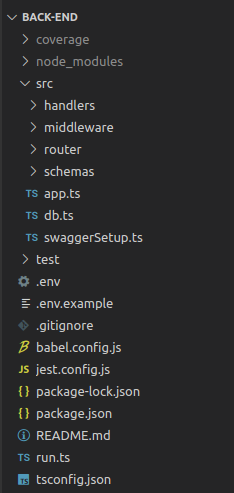
\includegraphics[scale=0.5]{structure.png}
        \end{center}
    \item[] Nella \textbf{root} del progetto troviamo il file principale che esegue il server e la connessione al database, avvalendosi di vari file presenti nella cartella \textbf{src}.
    \item[] Sempre nella \textbf{root} sono presenti i vari file di configurazione del server necessari alla corretta esecuzione del server e del testing di cui parleremo in una successiva sezione.
    \item[] La cartella \textbf{src} contiene i due file principali eseguiti dal main \textbf{run.ts}, \textbf{app.ts} e \textbf{db.ts}, e una serie di sottocartelle.
    \item[] \textbf{Handlers} contiene le funzioni che elaborano le richieste costruendo le risposte da inviare al front-end.
    \item[] \textbf{Middleware} contiene funzioni di supporto agli handlers.
    \item[] \textbf{Router} contiene i router per gestire le richieste in arrivo e invocare l'handler appropriato.
    \item[] \textbf{Schemas} contiene le strutture date utilizzate.
\end{description}
\clearpage
\subsection{Project Dependencies}
\begin{description}
    \item[] Sono stati utilizzati e aggiunti al file \textbf{package.json} e seguenti moduli Node:
        \begin{itemize}
            \item bcrypt
            \item dotenv
            \item express
            \item jsonwebtoken
            \item mongoose
            \item swagger-jsdoc
            \item swagger-ui-express
            \item ts-node
            \item typescript
        \end{itemize}
    \item[] Sono presenti, sempre nel file \textbf{package.json}, le seguenti dipendenze di development:
        \begin{itemize}
            \item @babel/core
            \item @babel/preset-env
            \item @babel/preset-typescript
            \item @types/bcrypt
            \item @types/express
            \item @types/jest
            \item @types/jsonwebtoken
            \item @types/swagger-jsdoc
            \item @types/swagger-ui-express
            \item babel-jest
            \item jest
            \item node-fetch
            \item nodemon
            \item ts-jest
        \end{itemize}
\end{description}
\clearpage
\subsection{Project Data}
\begin{description}
    \item[] Per la gestione dati dell'applicazione viene usato il database \href{https://www.mongodb.com/atlas}{MongoDB Atlas}. Sono state definite due strutture principali: \textbf{User} e \textbf{Evento}.
    \item[] Il progetto utilizza inoltre un databese (e server) separato unicamente per il testing per evitare di mescolare deployment e testing.
    \item[] Per descrivere documenti di tipo \textbf{User} è stata definita la seguente interfaccia \hyperref[img:3]{(Figura 3)}:
    \item[] \label{img:3} \begin{center}
            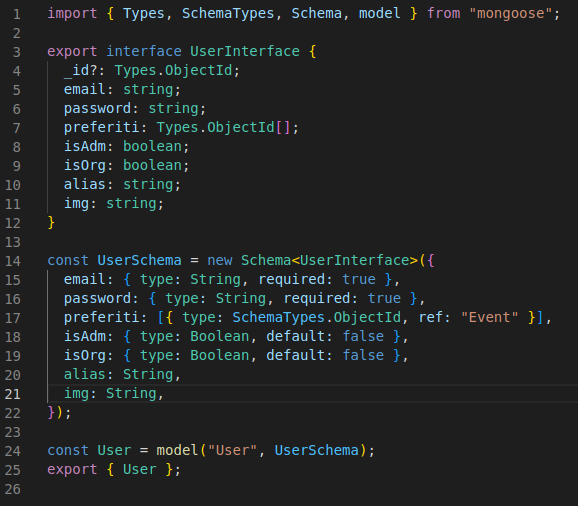
\includegraphics[scale=0.5]{UserInterface.png}
        \end{center}
        \clearpage
    \item[] Per descrivere documenti di tipo \textbf{Evento} è stata definita la seguente interfaccia \hyperref[img:4]{(Figura 4)}:
    \item[] \label{img:4} \begin{center}
            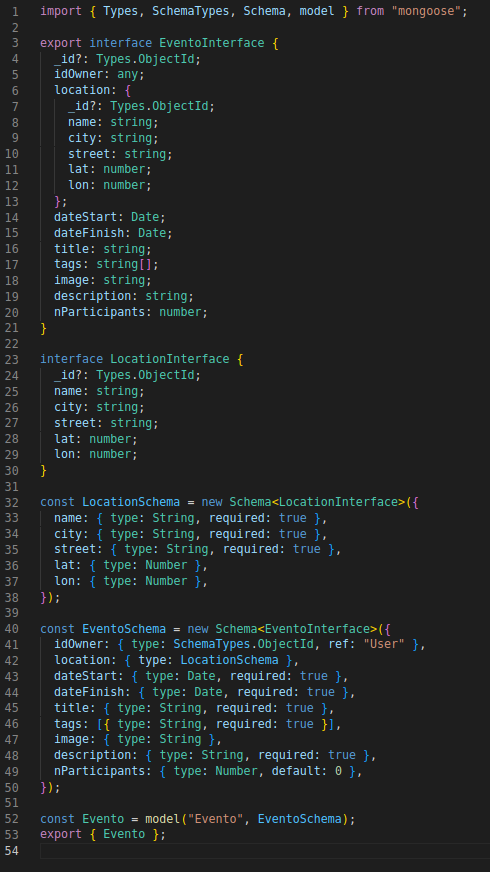
\includegraphics[scale=0.5]{EventoInterface.png}
        \end{center}
    \item[] Come si può notare è stata definita un'interfaccia di supporto \textbf{location} per definire la location dell'Evento.
\end{description}
\clearpage
\subsection{Project APIs}
\subsubsection{Resources Extraction from the Class Diagram}
\begin{description}
    \item[] Dal Class Diagram sono state estratte le risorse rappresentate in \hyperref[img:5]{Figura 5}.
    \item[] Identifichiamo \textbf{User} e \textbf{Evento} (con \textbf{Location} a supporto) da cui accediamo a varie richieste eseguibili dall'app.
    \item[] Per \textbf{User} abbiamo lato back-end le risorse \textbf{new} (per creare un nuovo utente), \textbf{login} (per identificarci univocamente) e \textbf{delete} (per eliminare il nostro account), mentre lato front-end la risorsa \textbf{logout} (per effettuare il logout dall'app).
    \item[] Per \textbf{Evento} abbiamo lato back-end le risorse \textbf{all} (per richiedere l'elenco completo degli eventi nel DB), \textbf{event} (per richiedere un singolo evento in base all'id), \textbf{new} (per creare un nuovo evento), \textbf{modify} (per modificare un evento esistente), \textbf{delete} (per eliminare un evento), \textbf{tag} (per effettuare una ricerca tramite tag), \textbf{period} (per effettuare una ricerca a livello giornaliero, settimanale o mensile), \textbf{preferito} (per aggiungere o rimuovere un evento dai preferiti).
    \item[] \label{img:5} \begin{center}
            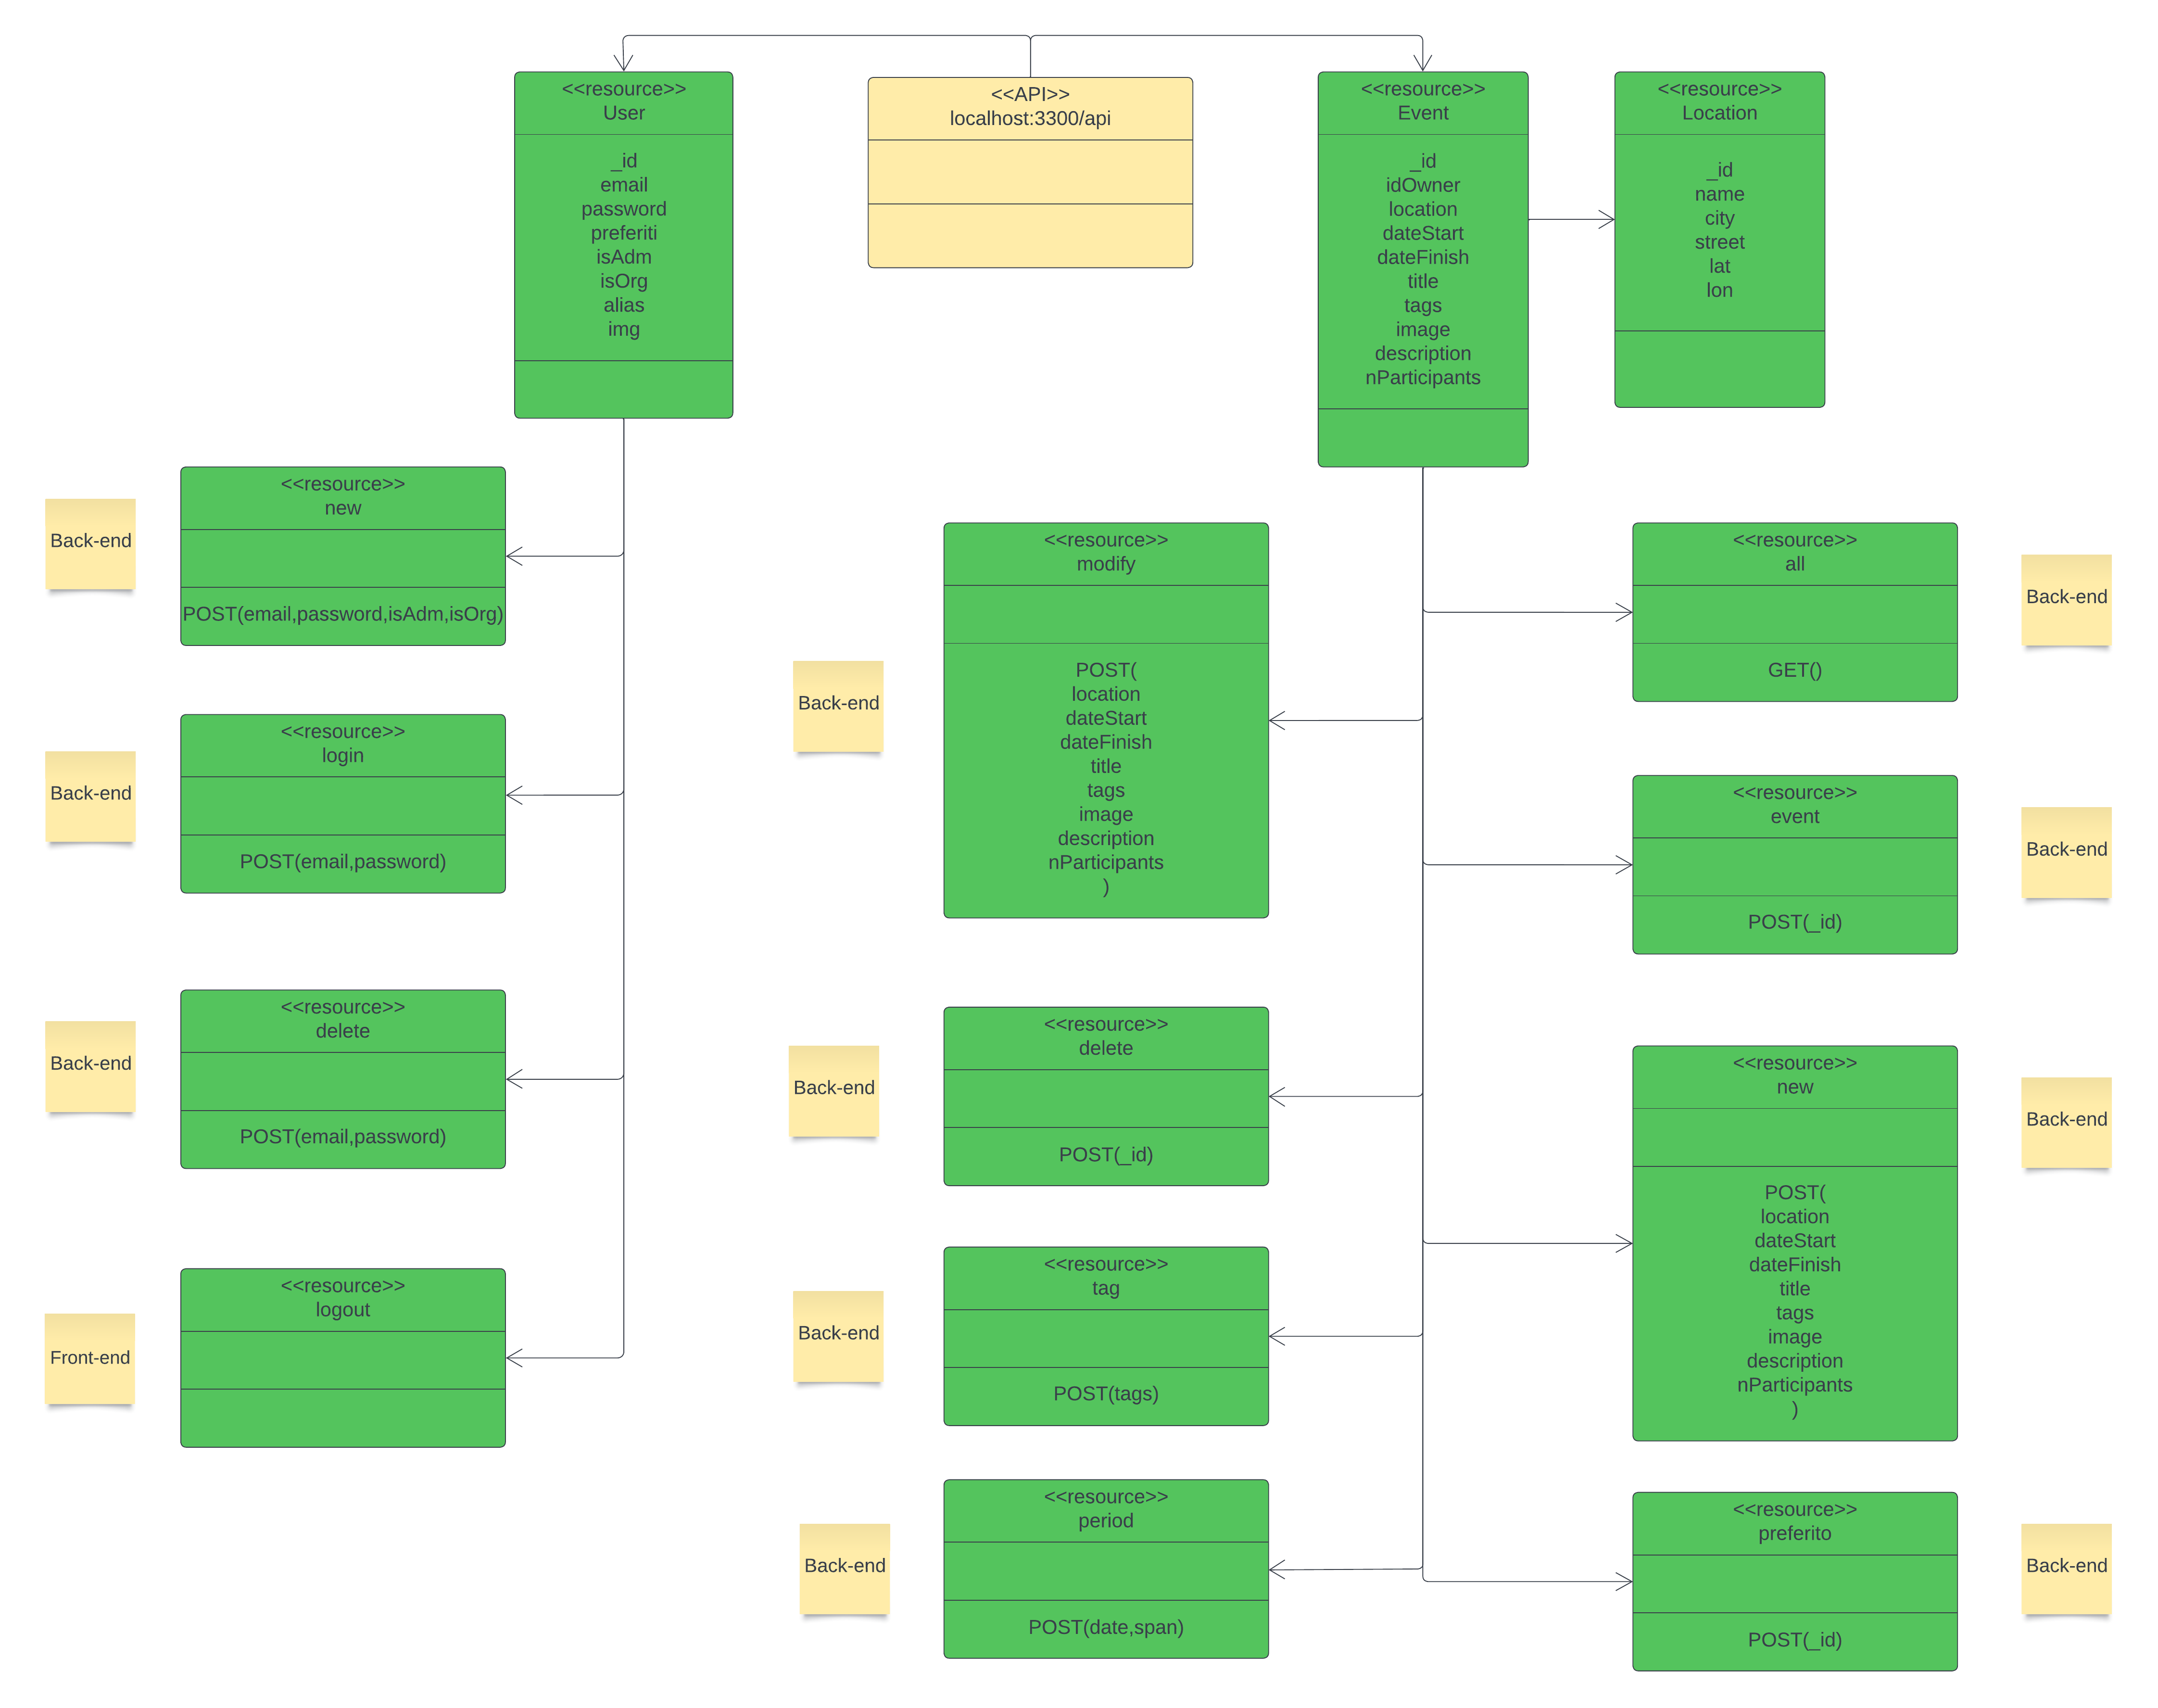
\includegraphics[scale=0.4]{resources.png}
        \end{center}
\end{description}
\subsubsection{Resources Models}
\begin{description}
    \item[] Identificate le risorse è stato costruito un diagramma delle API per identificare i request e response body e le varie tipologie di risposta che possiamo aspettarci dalle API.
        \clearpage
    \item[] Osserviamo in \hyperref[img:6]{Figura 6} il diagramma inerente agli User:
    \item[] \label{img:6} \begin{center}
            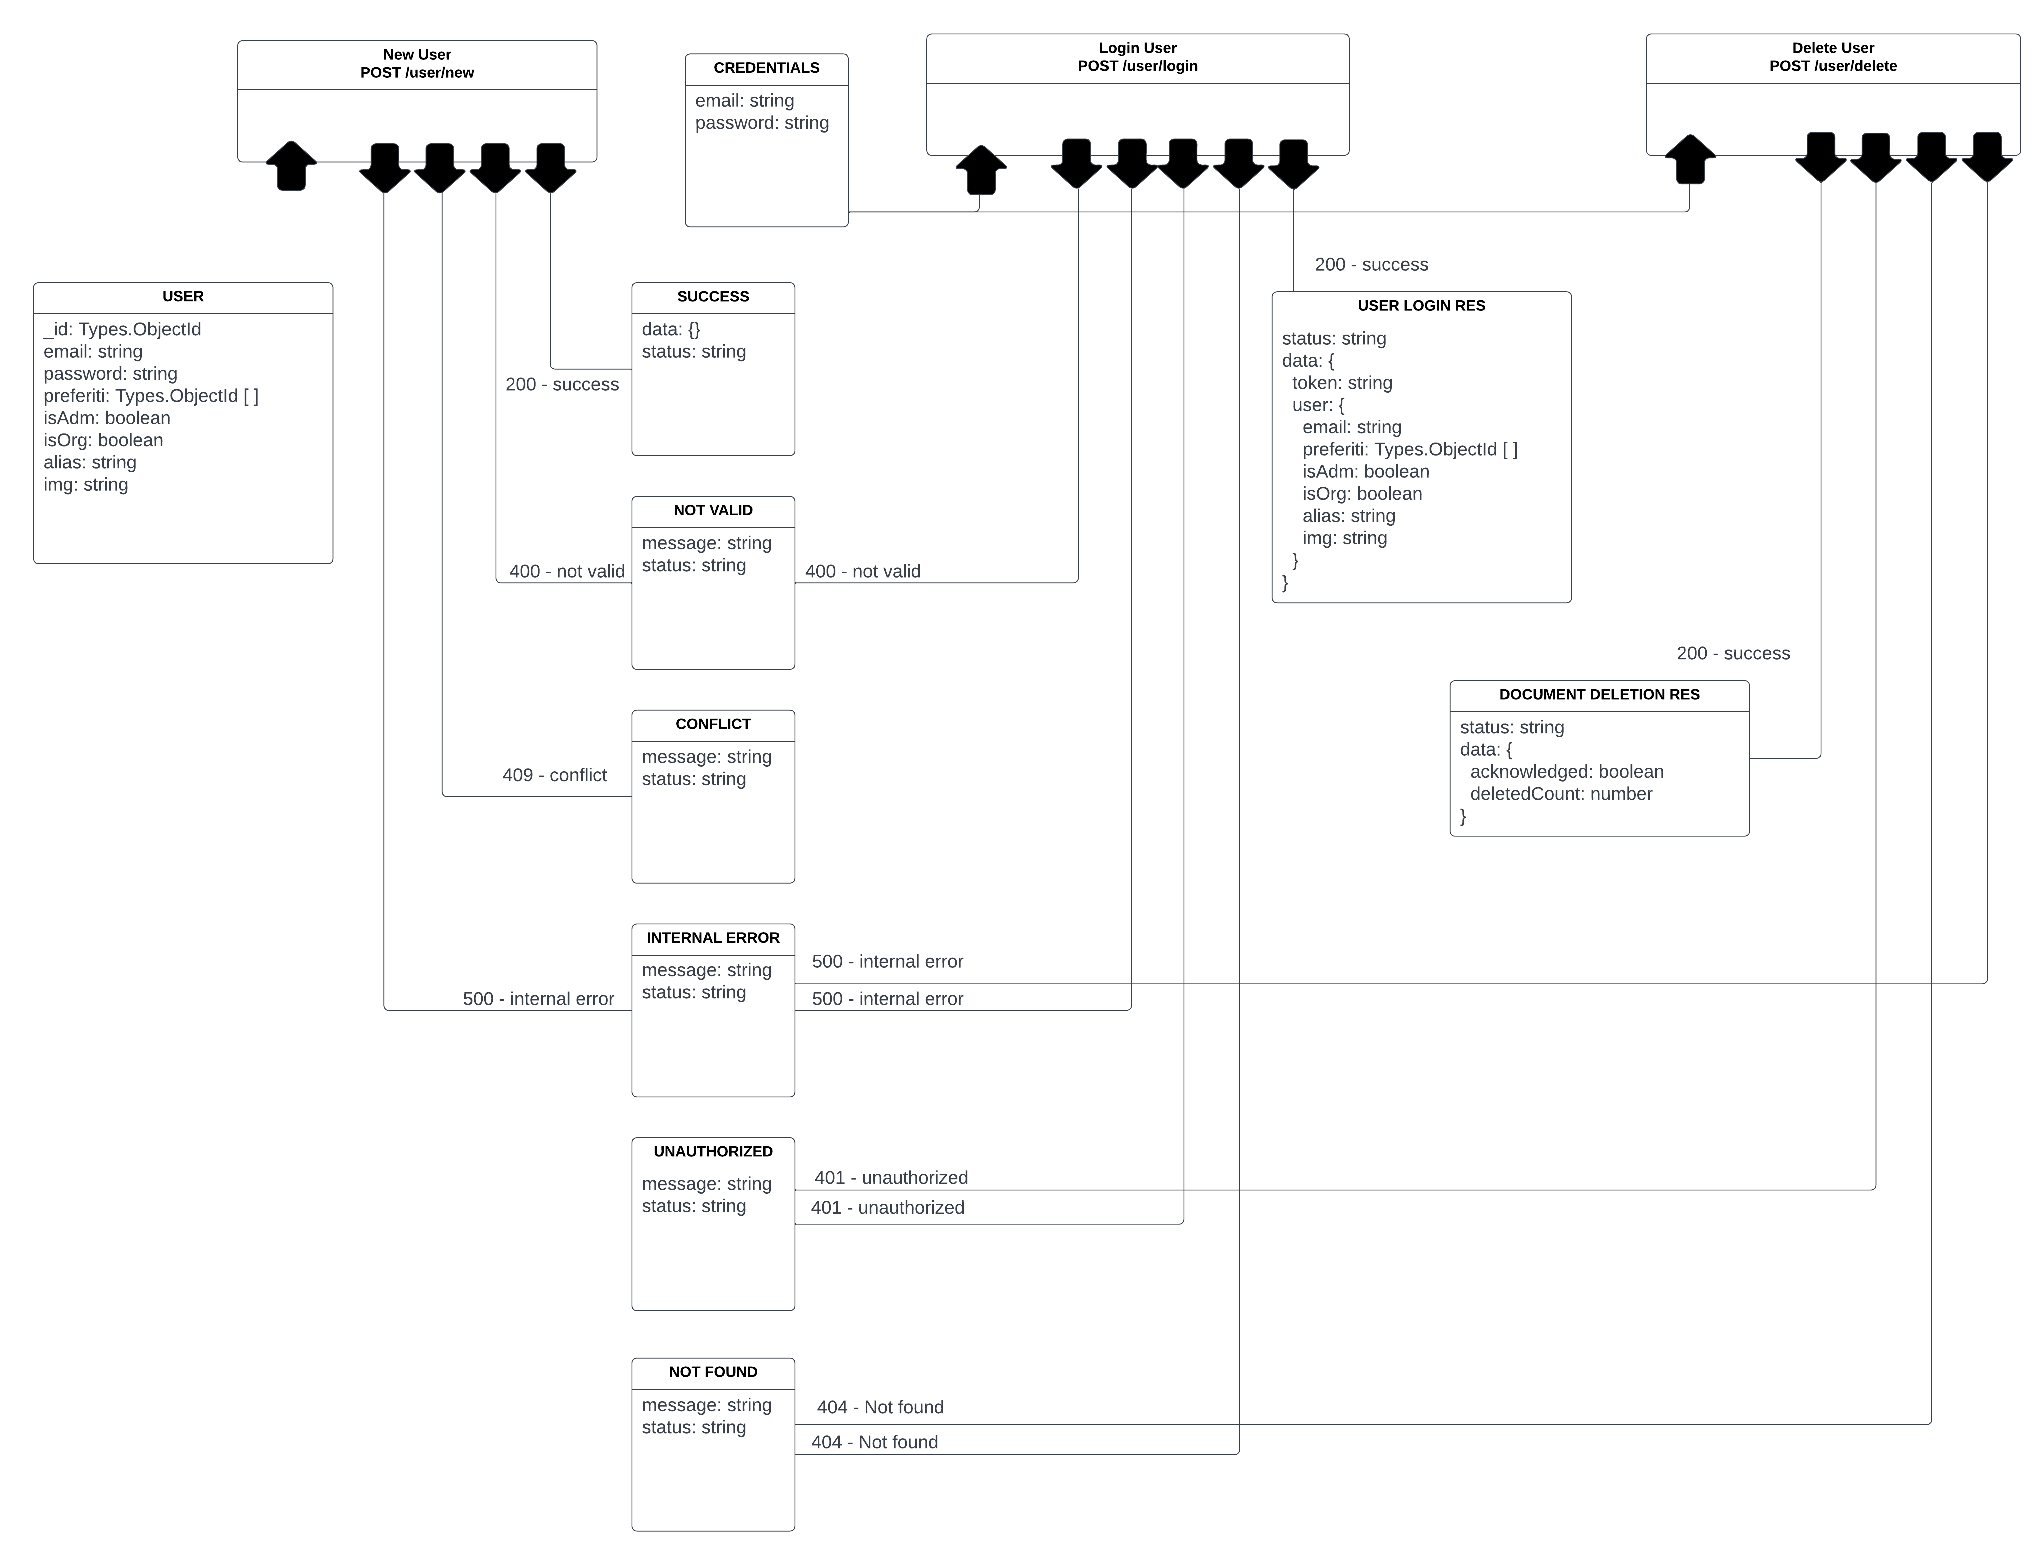
\includegraphics[scale=0.9]{userResources.png}
        \end{center}
        \clearpage
    \item[] Osserviamo in \hyperref[img:7]{Figura 7} il diagramma inerente agli Eventi (parte 1):
    \item[] \label{img:7} \begin{center}
            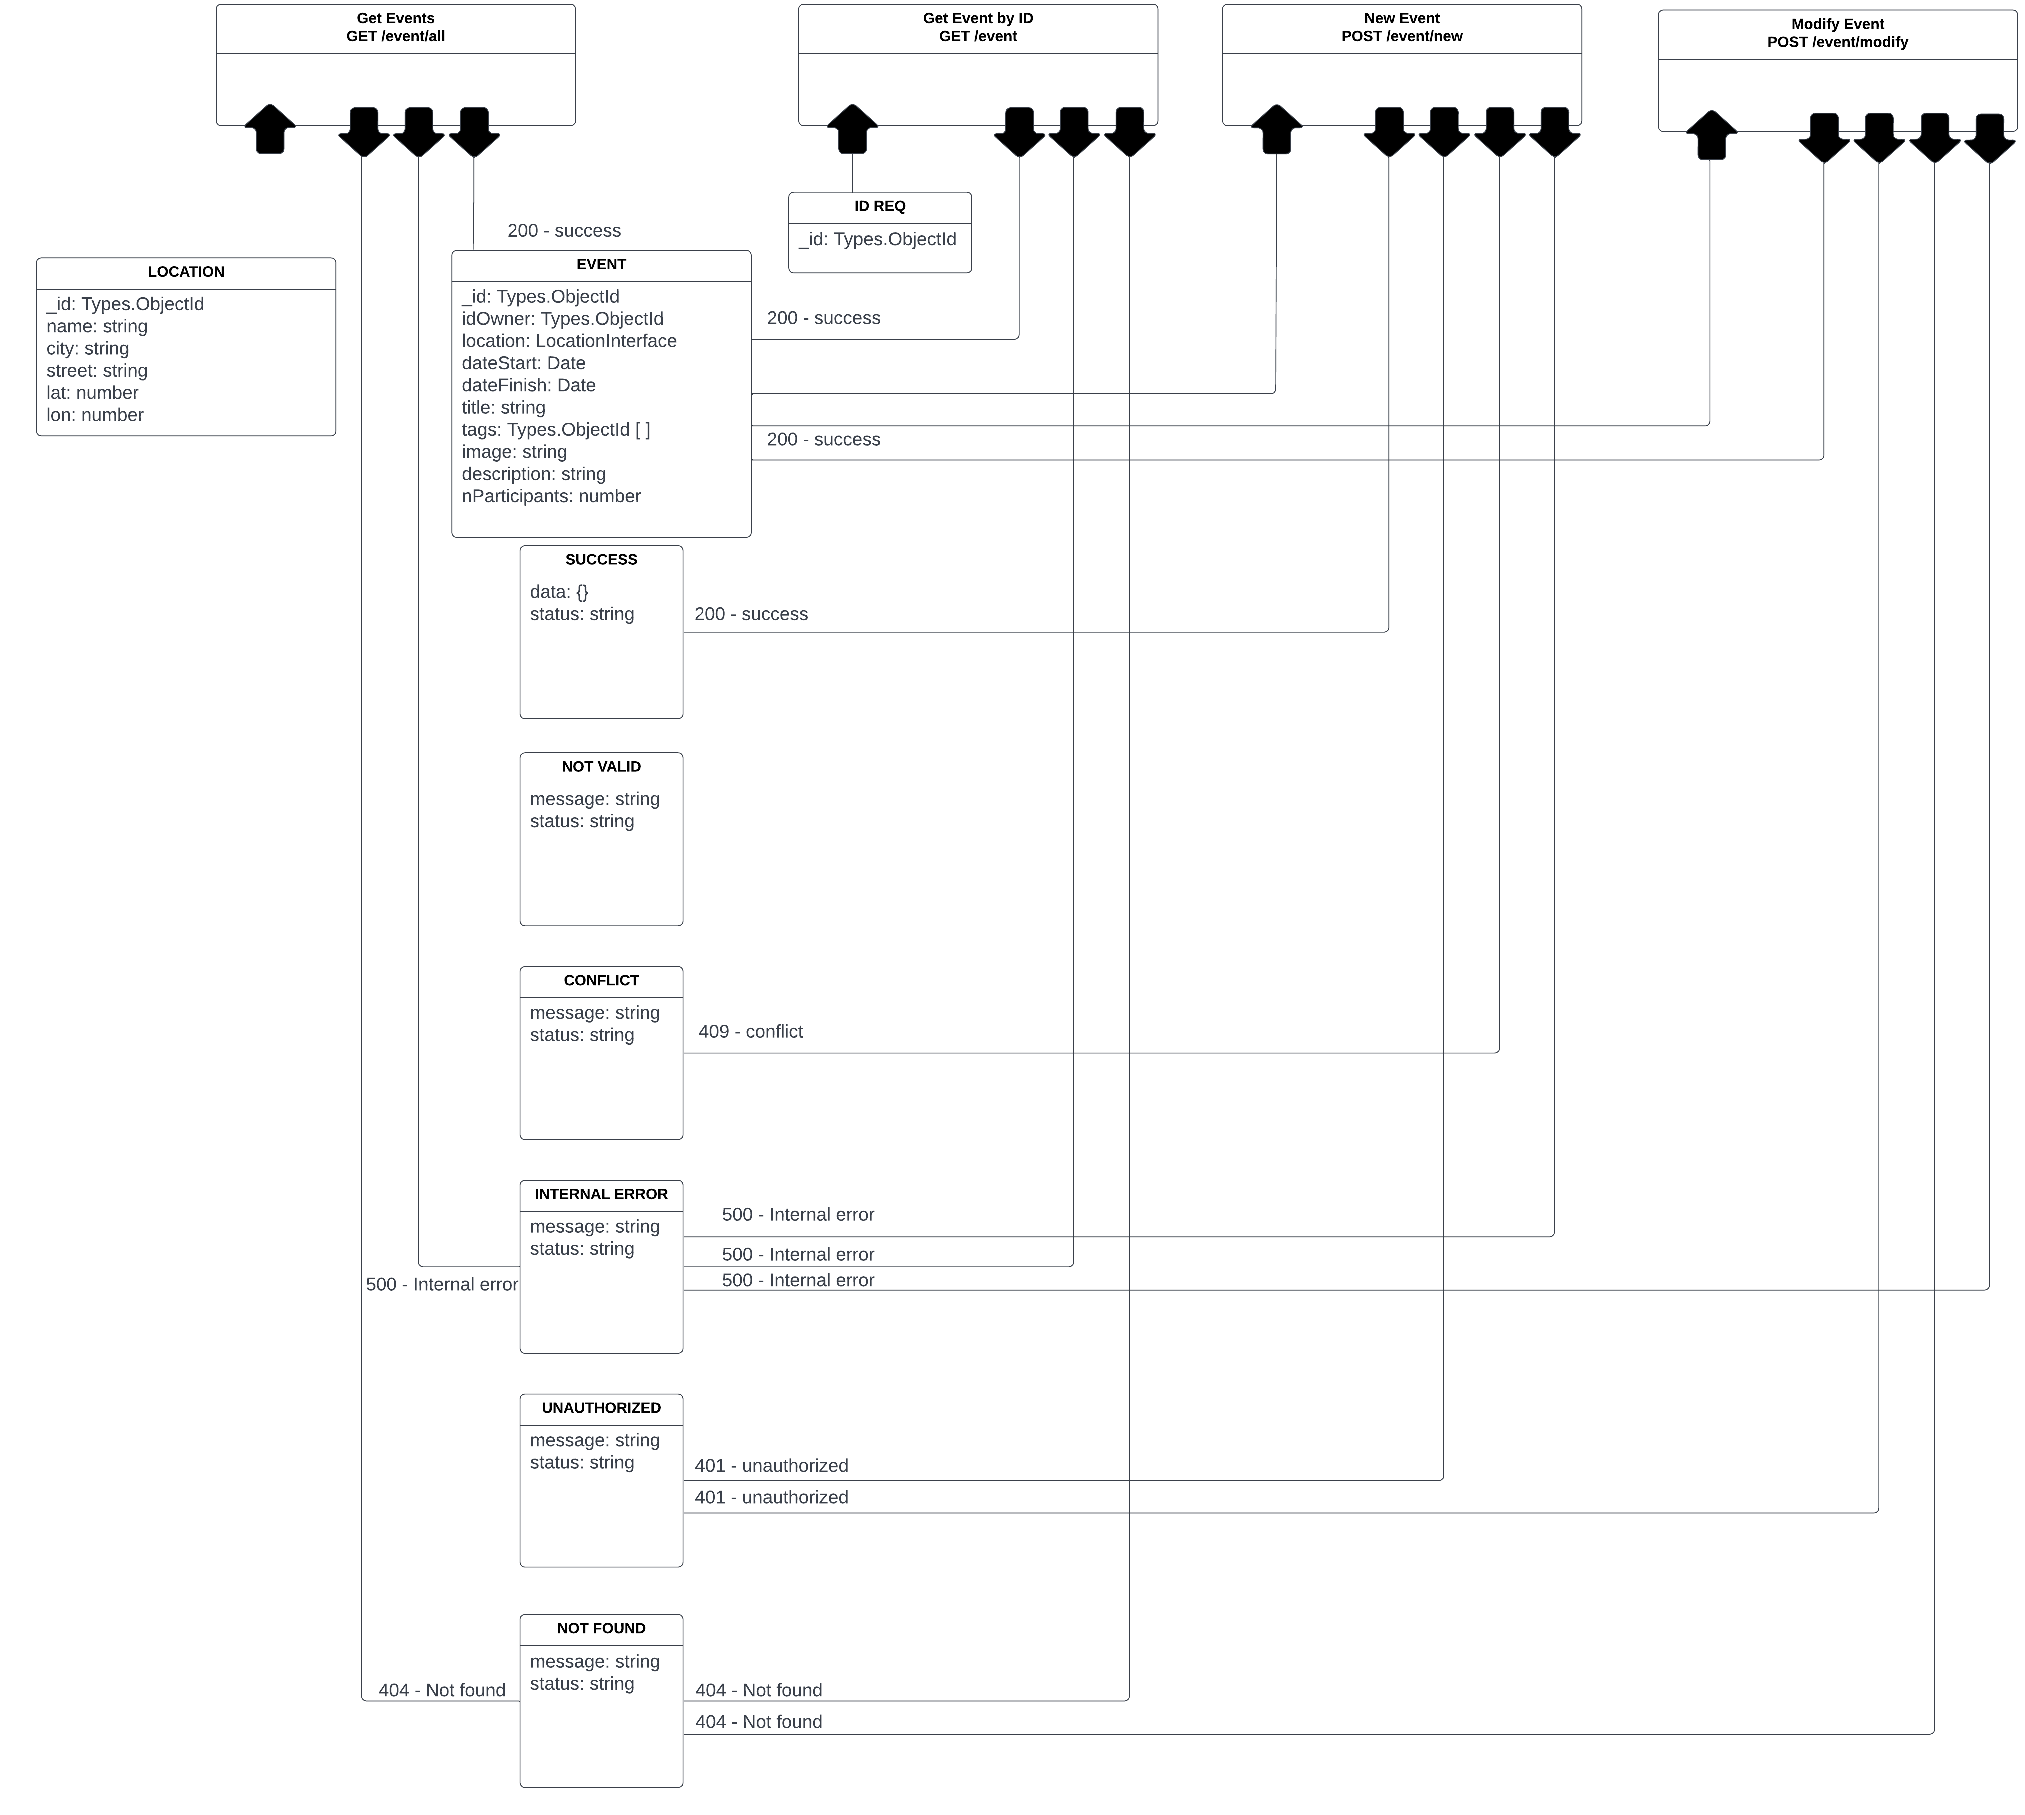
\includegraphics[scale=0.9]{eventResources1.png}
        \end{center}
        \clearpage
    \item[] Osserviamo in \hyperref[img:8]{Figura 8} il diagramma inerente agli Eventi (parte 2):
    \item[] \label{img:8} \begin{center}
            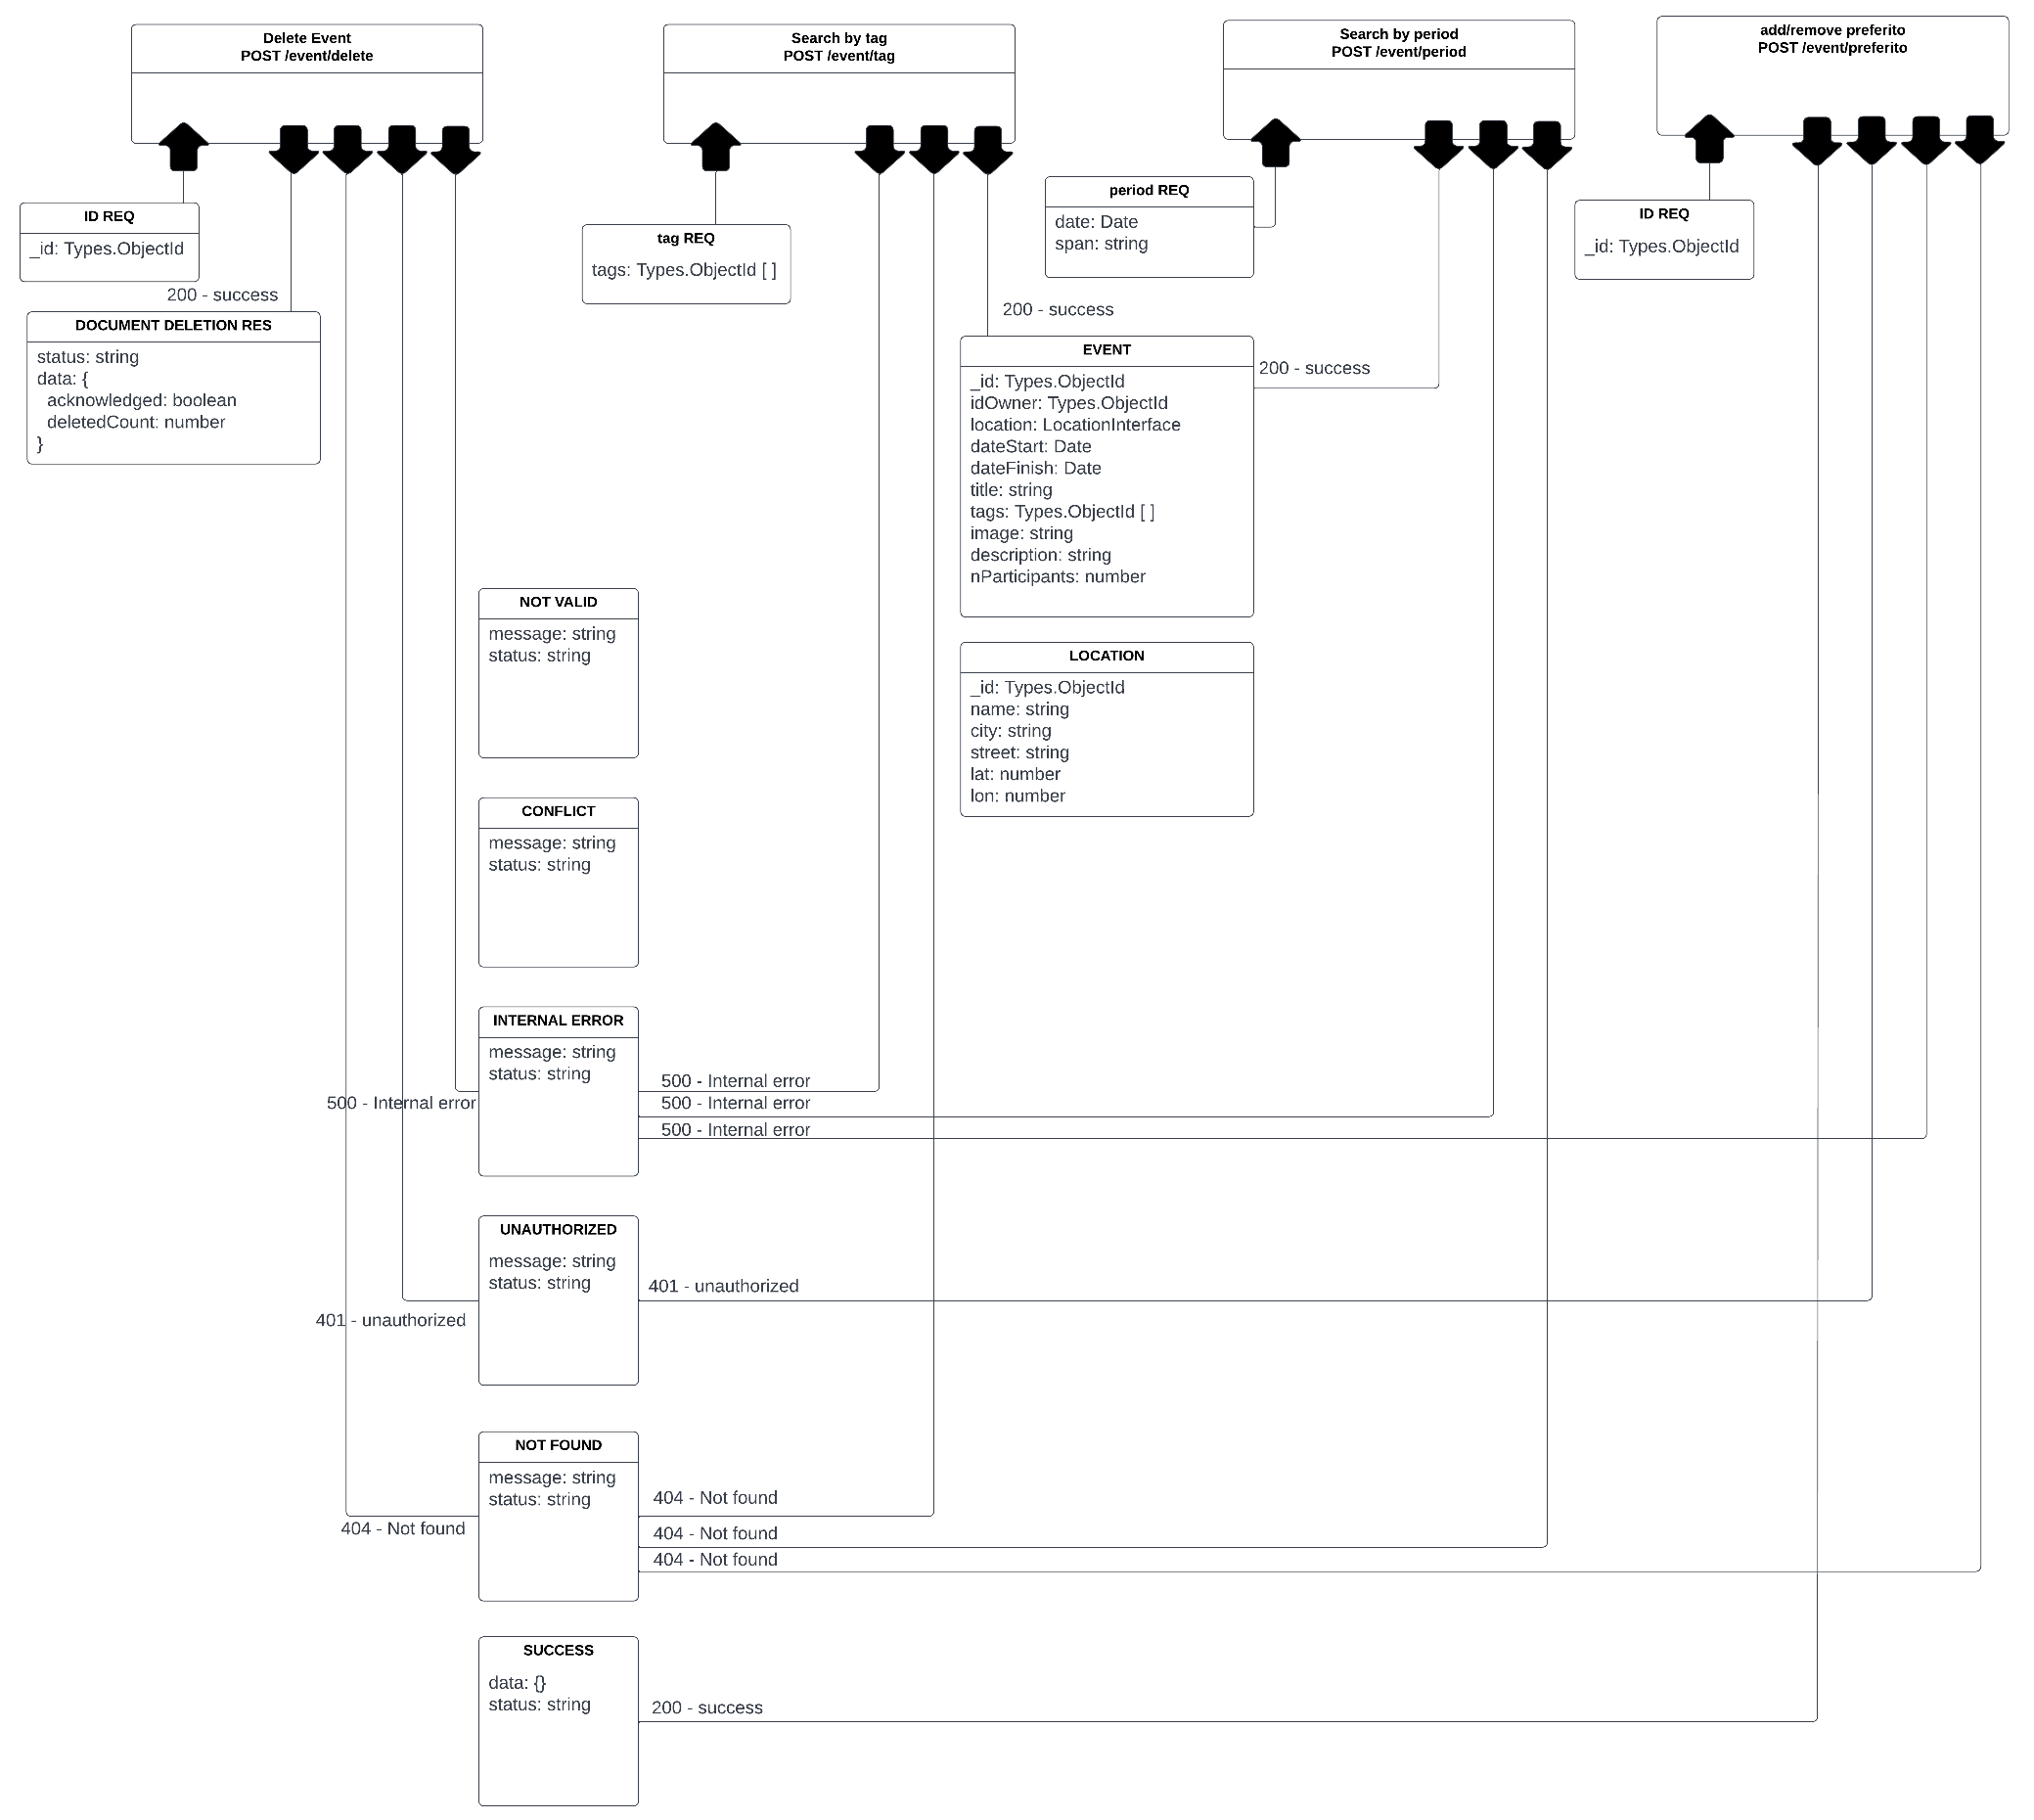
\includegraphics[scale=0.9]{eventResources2.png}
        \end{center}
\end{description}
\clearpage
\subsection{Sviluppo API}
\begin{description}
    \item[] Le API vengono gestite dai router presenti nella cartella router dell'app.
    \item[] \begin{center}
            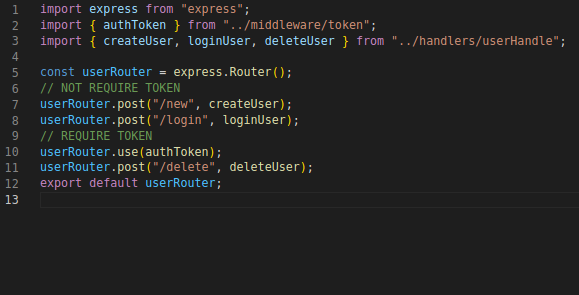
\includegraphics[scale=0.5]{userRouter.png}
        \end{center}
    \item[] \begin{center}
            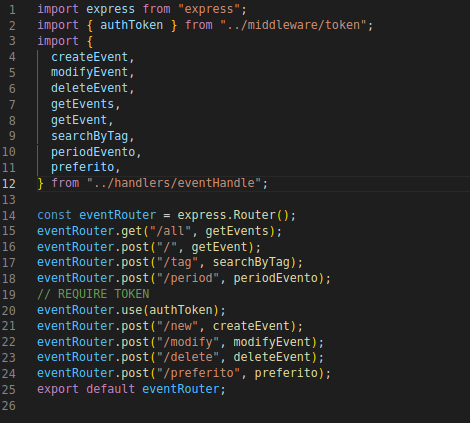
\includegraphics[scale=0.5]{eventRouter.png}
        \end{center}
\end{description}
\clearpage
\subsubsection{Creazione nuovo User}
\begin{description}
    \item[] Tramite questa API è possibile creare un nuovo utente, purché la mail fornita non sia già utilizzata da un altro utente (in questo caso l'app ci risponderà con un errore 409).
    \item[] L'utente deve inviare sia una mail che una password, in caso contrario l'app risponderà con un errore 400.
    \item[] In caso di successo riceveremo un messaggio di conferma con codice 200.
    \item[] \begin{center}
            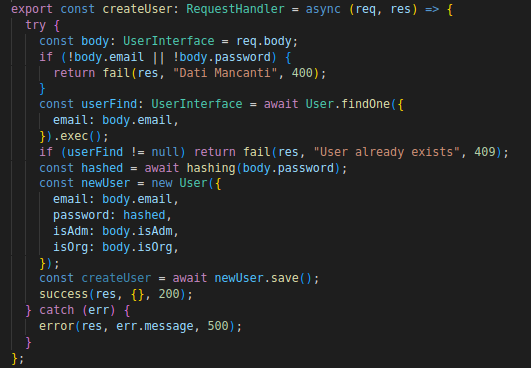
\includegraphics[scale=0.5]{newUser.png}
        \end{center}
\end{description}
\clearpage
\subsubsection{Login User}
\begin{description}
    \item[] Tramite questa API lo User può effettuare il login all'app utilizzando le credenziali con cui è stato creato l'utente.
    \item[] Se la richiesta dovesse andare a buon fine l'app risponderà con i dati principali dell'utente (email, array dei preferiti, eventuali poteri superiori da admin o organizzatore) e con un token JWT che lo User utilizzerà per tutte quelle richieste che necessitano di verifica dei poteri posseduti.
    \item[] L'utente deve inviare sia una mail che una password, in caso contrario l'app risponderà con un errore 400.
    \item[] Se la password dovesse essere scorretta l'app risponderà con un messaggio di errore con codice 401.
    \item[] Se non venisse trovato nessun utente identificato dall'email fornita l'app risponderà con un messaggio di errore con codice 404.
    \item[] \begin{center}
            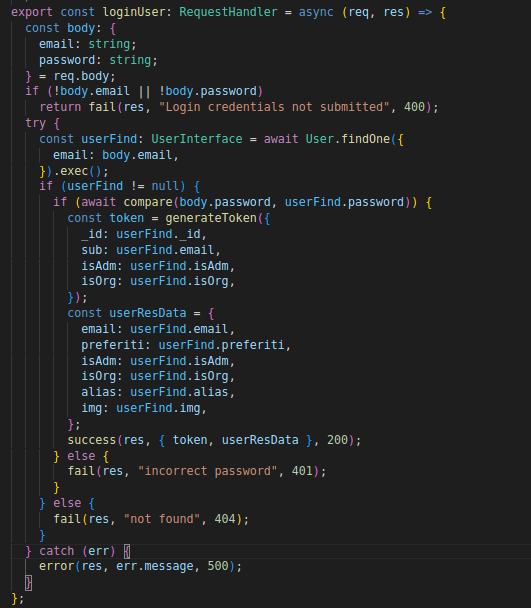
\includegraphics[scale=0.5]{loginUser.png}
        \end{center}
\end{description}
\clearpage
\subsubsection{Eliminazione User}
\begin{description}
    \item[] Tramite questa API è possibile elimiare il proprio account inserendo mail e password (oppure, se si possiedono poteri da amministratore, eliminare un account fornendone solo la mail).
    \item[] In caso di successo l'app risponderà con un messaggio di conferma con codice 200.
    \item[] Essendo necesasrio il JWT per compiere questa operazione in caso di errore dell'elaborazione dello stesso riceveremo in risposta un messaggio di errore con codice 401.
    \item[] Immettendo una email incorretta l'app, non trovando lo user, risponderà con un messaggio di errore con codice 404.
    \item[] \begin{center}
            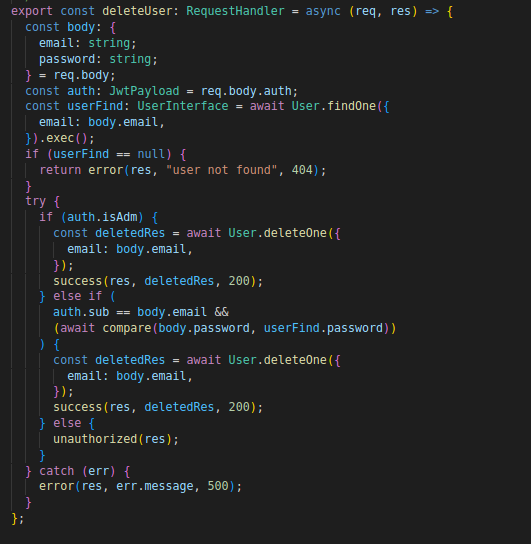
\includegraphics[scale=0.5]{deleteUser.png}
        \end{center}
\end{description}
\subsubsection{Stampa tutti gli Eventi}
\begin{description}
    \item[] Tramite questa API è possibile ottenere l'elenco di tutti gli eventi salvati nel DB.
    \item[] Nel caso in cui ci fossero effettivamente degli eventi salvati l'app ce li restituirebbe sotto forma di array.
    \item[] In caso contrario riceveremo un messaggio di errore con codice 404.
    \item[] \begin{center}
            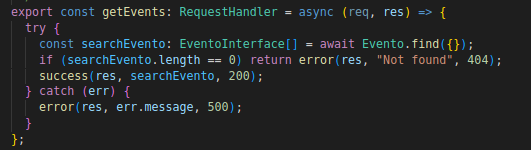
\includegraphics[scale=0.5]{allEvent.png}
        \end{center}
\end{description}
\clearpage
\subsubsection{Stampa singolo Evento}
\begin{description}
    \item[] Tramite questa API è possibile ottenere informazioni riguardo ad un evento selezionandolo tramite ID.
    \item[] Se l'ID identifica effettivamente un evento lo otterremo in risposta, in caso contrario riceveremo un messaggio di errore con codice 404.
    \item[] \begin{center}
            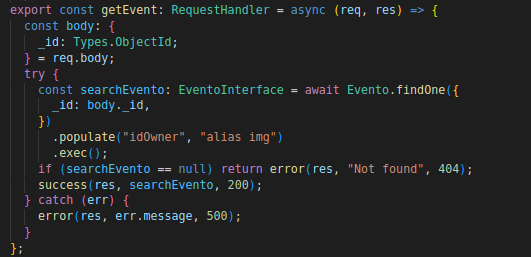
\includegraphics[scale=0.5]{getEvent.png}
        \end{center}
\end{description}
\subsubsection{Creazione nuovo Evento}
\begin{description}
    \item[] Tramite questa API è possibile creare un nuovo evento fornendone i dati necessari se si dispone dell'autorizzazione necessaria (essere organizzatori).
    \item[] In caso di successo si riceverà un messaggio di conferma con codice 200.
    \item[] Se il token fornito per l'autorizzazione non ci identificasse come organizzatori l'app ci risponderebbe con un messaggio di errore con codice 401.
    \item[] Non è possibile creare un evento con lo stesso titolo e la stessa esatta data di inizio, se stessimo cercando di creare un evento infrangendo questa regola l'app ci risponderebbe con un messaggio di errore con codice 409.
    \item[] \begin{center}
            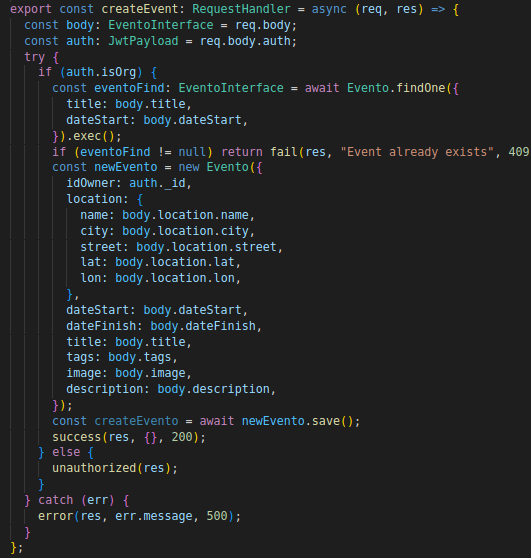
\includegraphics[scale=0.5]{newEvent.png}
        \end{center}
\end{description}
\clearpage
\subsubsection{Modifica Evento}
\begin{description}
    \item[] Tramite questa API è possibile modificare un evento se ne siamo noi stessi il creatore (ci identifichiamo tramite JWT) o se siamo un admin. È necessario fornire i dati da modificati.
    \item[] In caso di successo l'app ci restituirà l'evento modificato.
    \item[] Se non possedessimo l'autorizzazione necessaria riceveremmo dall'app un messaggio di errore con codice 401.
    \item[] Se ci fosse un errore con l'id fornito (che identifica l'evento nel DB) e quindi l'app non riuscisse a trovare nessun evento da modificare, riceveremmo in risposta un messaggio di errore con codice 404.
    \item[] \begin{center}
            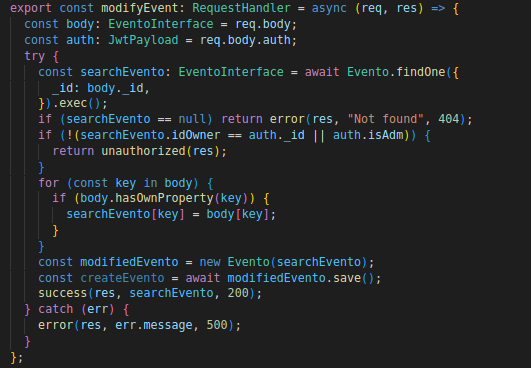
\includegraphics[scale=0.5]{modifyEvent.png}
        \end{center}
\end{description}
\subsubsection{Eliminazione Evento}
\begin{description}
    \item[] Tramite questa API è possibile eliminare un nostro evento (o un evento qualsiasi se siamo admin).
    \item[] La mancanza di autorizzazione necessaria comporta un messaggio di errore con codice 401 in risposta.
    \item[] Se l'ID non dovesse corrispondere ad alcun evento riceveremmo in risposta un messaggio di errore con codice 404.
    \item[] \begin{center}
            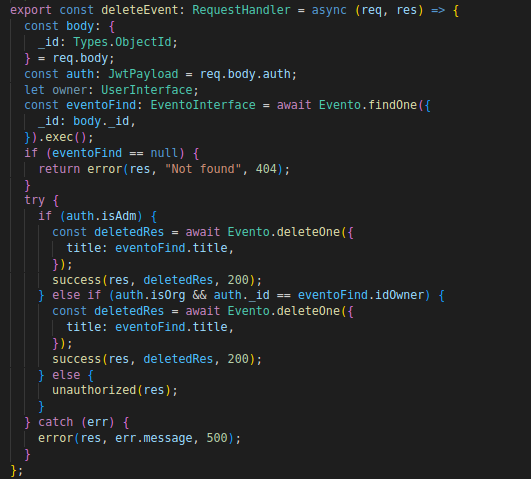
\includegraphics[scale=0.5]{deleteEvent.png}
        \end{center}
\end{description}
\clearpage
\subsubsection{Ricerca per Tag}
\begin{description}
    \item[] Tramite questa API è possibile effettuare una ricerca per tag (singolo o molteplici).
    \item[] La richiesta ha successo se riceviamo in risposta l'elenco degli eventi con almeno un tag presente nell'array tag.
    \item[] Se l'elenco è vuoto la risposta sarà un messaggio di errore con codice 404.
    \item[] \begin{center}
            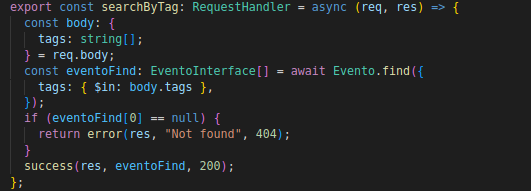
\includegraphics[scale=0.5]{tagEvent.png}
        \end{center}
\end{description}
\subsubsection{Ricerca per Periodo}
\begin{description}
    \item[] Tramite questa API è possibile effettuare una ricerca per periodo, ovvero fornita una data base è possibile richiedere all'app tutti gli eventi che iniziano o finiscono a partire da quella data fino al giorno/settimana/mese successivo.
    \item[] Come per la ricerca tramite tag o riceveremo un elenco di eventi o un messaggio di errore con codice 404.
    \item[] \begin{center}
            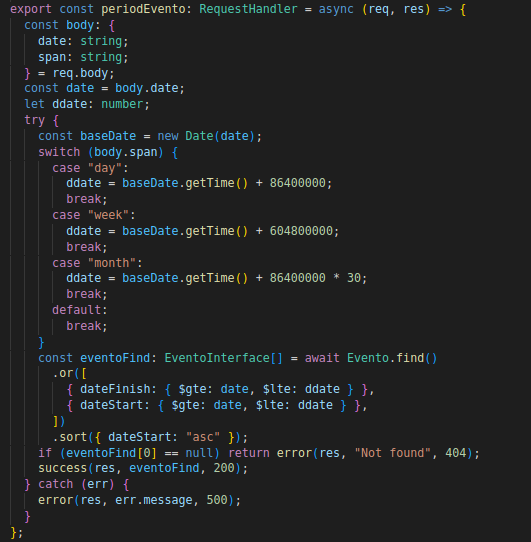
\includegraphics[scale=0.5]{periodoEvent.png}
        \end{center}
\end{description}
\clearpage
\subsubsection{Aggiunta/Rimozione dai Preferiti}
\begin{description}
    \item[] Tramite questa API è possibile aggiungere (se non è già presente) o rimuovere (se già è presente) un evento alla lista preferiti dell'utente.
    \item[] Un errore con il token di autenticazione comporta un messaggio di errore con codice 401.
    \item[] Se l'ID evento fornito non dovesse esistere riceveremmo un messaggio di errore con codice 404.
    \item[] \begin{center}
            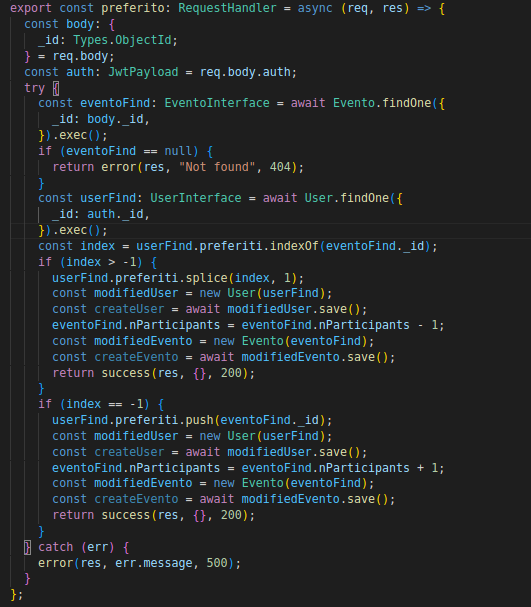
\includegraphics[scale=0.5]{preferitoEvent.png}
        \end{center}
\end{description}
\clearpage
\section{API Documentation}
\begin{description}
    \item[] Le API Locali, descritte nella sezione precedente, fornite dall'applicazione FenFesta sono state documentate utilizzando il modulo NodeJS chiamato Swagger UI Express.
    \item[] Così facendo, aprendo la pagina designata, il reperimento della documentazione relativa alle suddette API è facilmente consultabile da qualunque persona.
    \item[] Per poter generare l'endpoint dedicato alla presentazione delle API è stato utilizzato Swagger UI in quanto crea una pagina web dalle definizioni delle specifiche OpenAPI.
    \item[] Di seguito \hyperref[img:9]{(Figura 9)} viene mostrata la pagina web relativa alla documentazione che presenta le API utilizzabili dall'utente generico per la visualizzazione degli eventi, partecipazione e salvataggio dell'evento, oltre a quelle utilizzabili da un utente con autorizzazioni più elevate per la creazione, modifica e eliminazione di eventi.
    \item[] L'endpoint da invocare per raggiungere la seguente documentazione è: \url{http://localhost:3300/api-docs}.
    \item[] \label{img:9} \begin{center}
            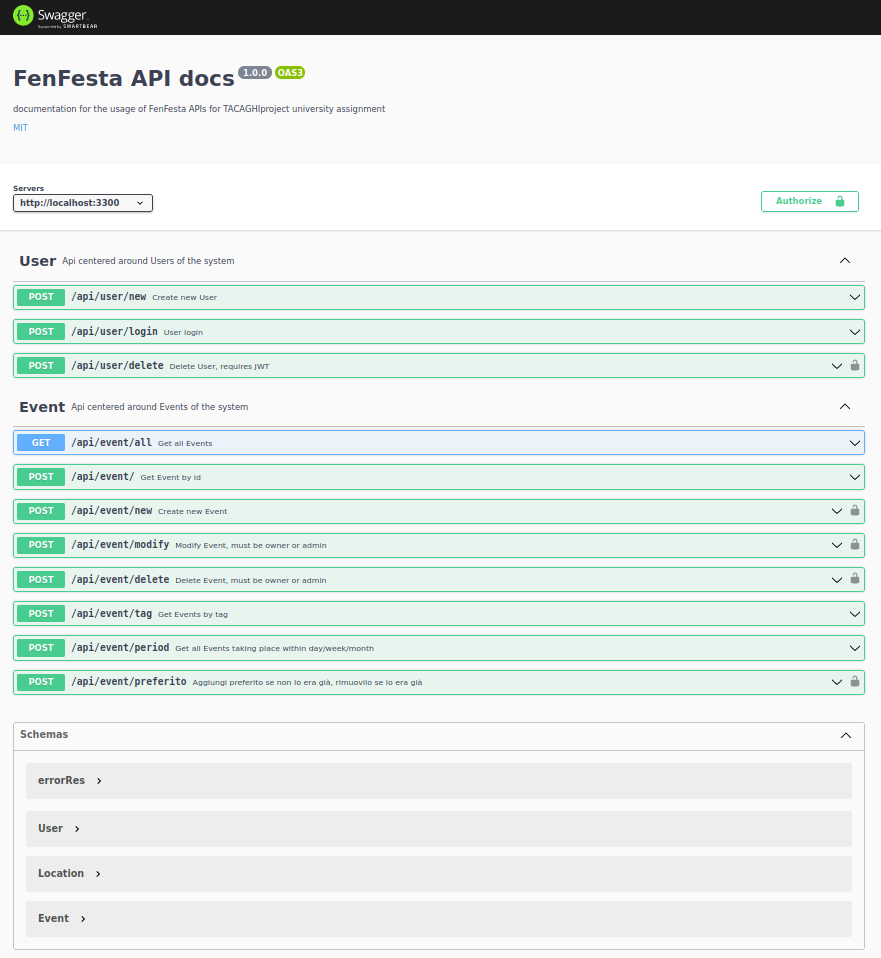
\includegraphics[scale=0.5]{documentazione.png}
        \end{center}
    \item[] Tramite la documentazione Swagger è possibile eseguire tutte le API fornite dall'app, comprese quelle che richiedono autenticazione tramite JWT (accessibile inserendo un token valido premento su Authorize).
\end{description}
\clearpage
\section{Front-End Implementation}
\begin{description}
    \item[] Il Font-End fornisce una visualizzazione grafica rispetto alle funzioni di:
        \begin{itemize}
            \item Creazione dell'Account
            \item Mappa Eventi
            \item Calendario Eventi
            \item Creazione di un Nuovo Evento
            \item Visualizzazione Evento
        \end{itemize}
    \item[] In particolare, tali funzioni sono suddivise nelle 5 schermate rinominate:
        \begin{itemize}
            \item Creazione Account
            \item Mappa
            \item Calendario
            \item Creazione
            \item Visualizza Evento
        \end{itemize}
\end{description}
\clearpage
\subsection{Mappa Eventi}
\begin{description}
    \item[] \begin{center}
            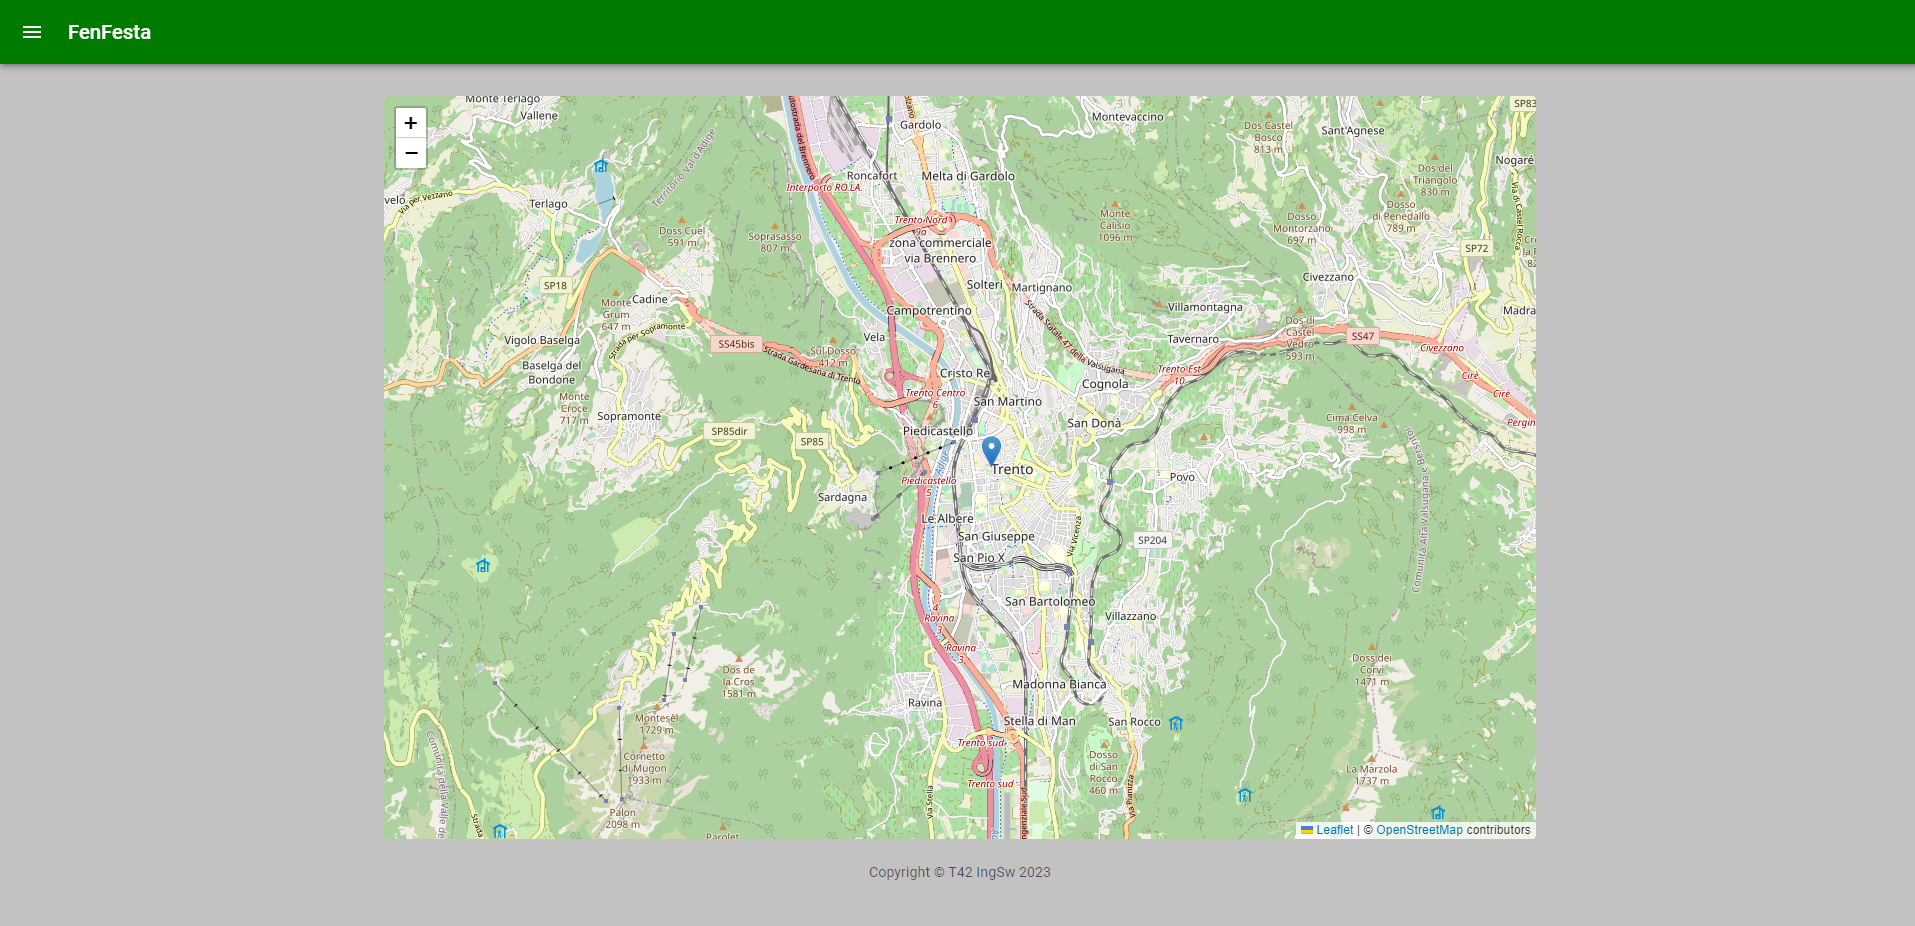
\includegraphics[scale=0.3]{Mappa_Eventi.png}
        \end{center}
    \item[] Nella sezione Mappa si può visualizzare una cartina interagibile, inserita grazie alle API di OpenStreetMap, nella quale sono posizionati dei marker che determinano la presenza di un Evento in quel punto. \\ Cliccandoci sopra si aprirà la sezione “Visualizza Evento”.
\end{description}
\subsection{Elenco Eventi}
\begin{description}
    \item[] \begin{center}
            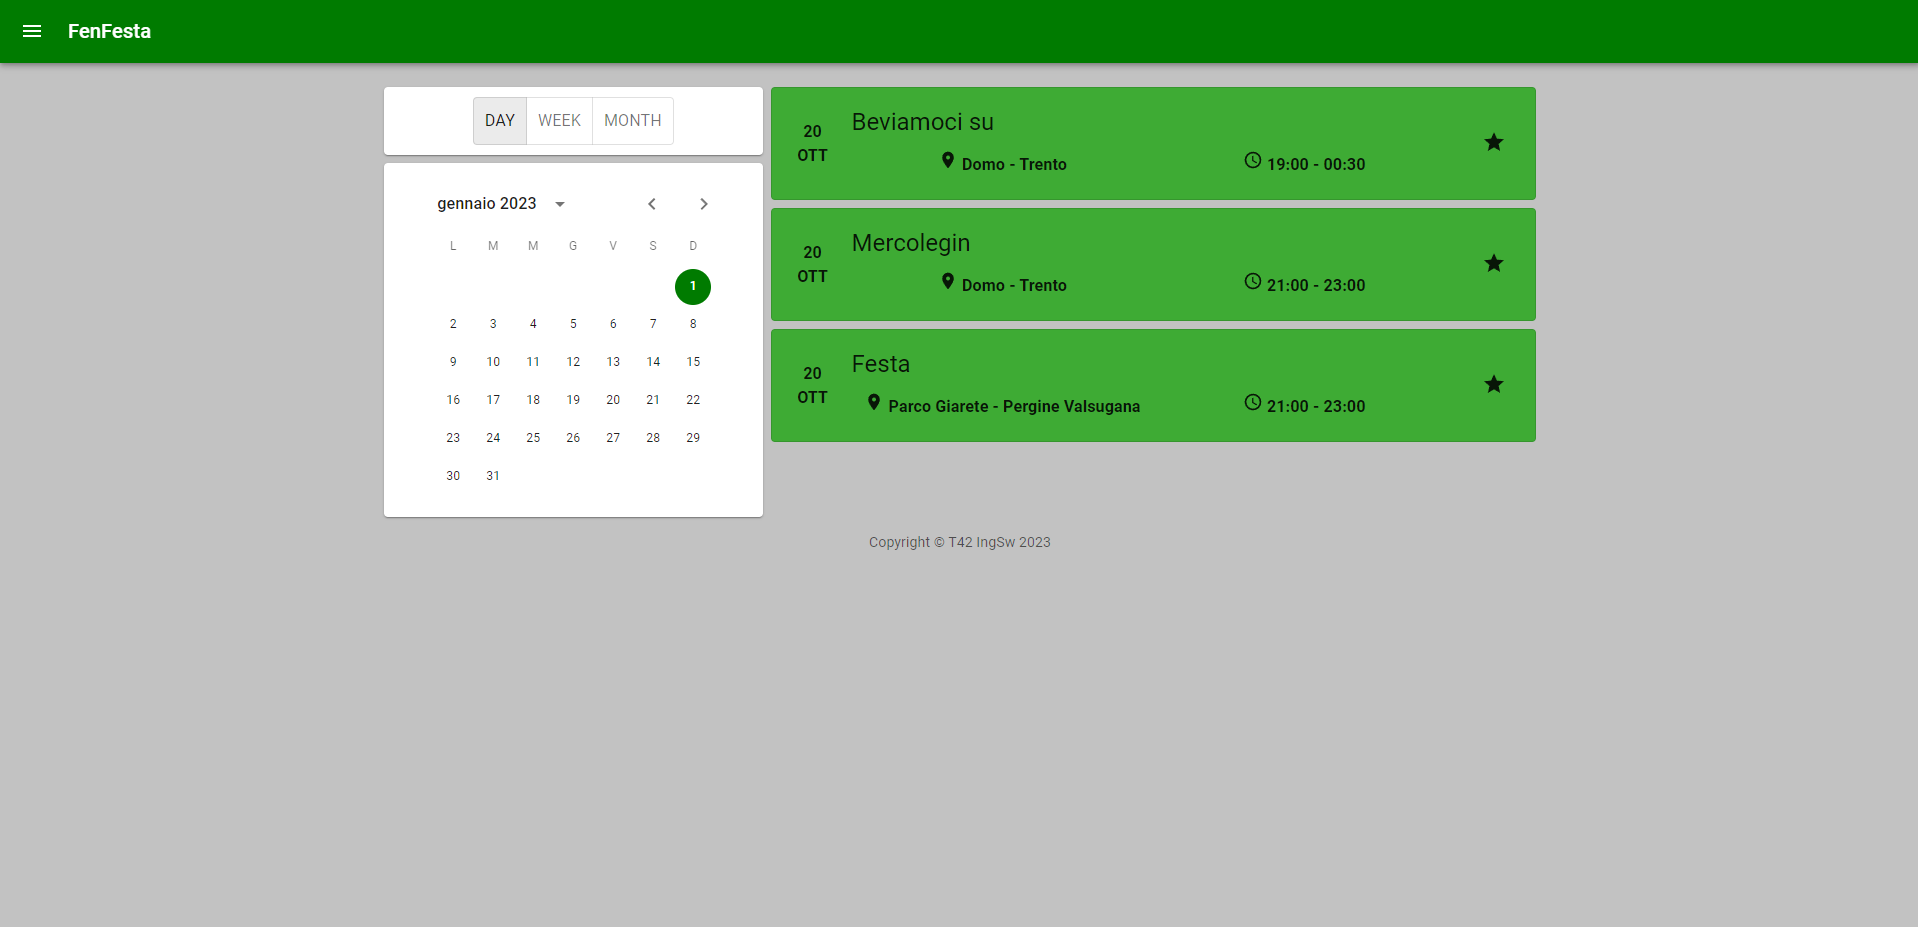
\includegraphics[scale=0.3]{Elenco_Eventi.png}
        \end{center}
    \item[] Nella schermata Calendario Eventi è disponibile un calendario con i giorni dell'anno ad accompagnare una lista di eventi disponibili giornalieri, settimanali o mensili
    \item[] Come nella Mappa, anche in questa schermata selezionando l'evento a cui si è interessati si aprirà la schermata di visualizzazione evento.
    \item[] Per selezionare l'Elenco o la Mappa è presente un menù laterale dove si può selezionare una delle due schermate
\end{description}
\clearpage
\subsection{Visualizza Evento}
\begin{description}
    \item[] \begin{center}
            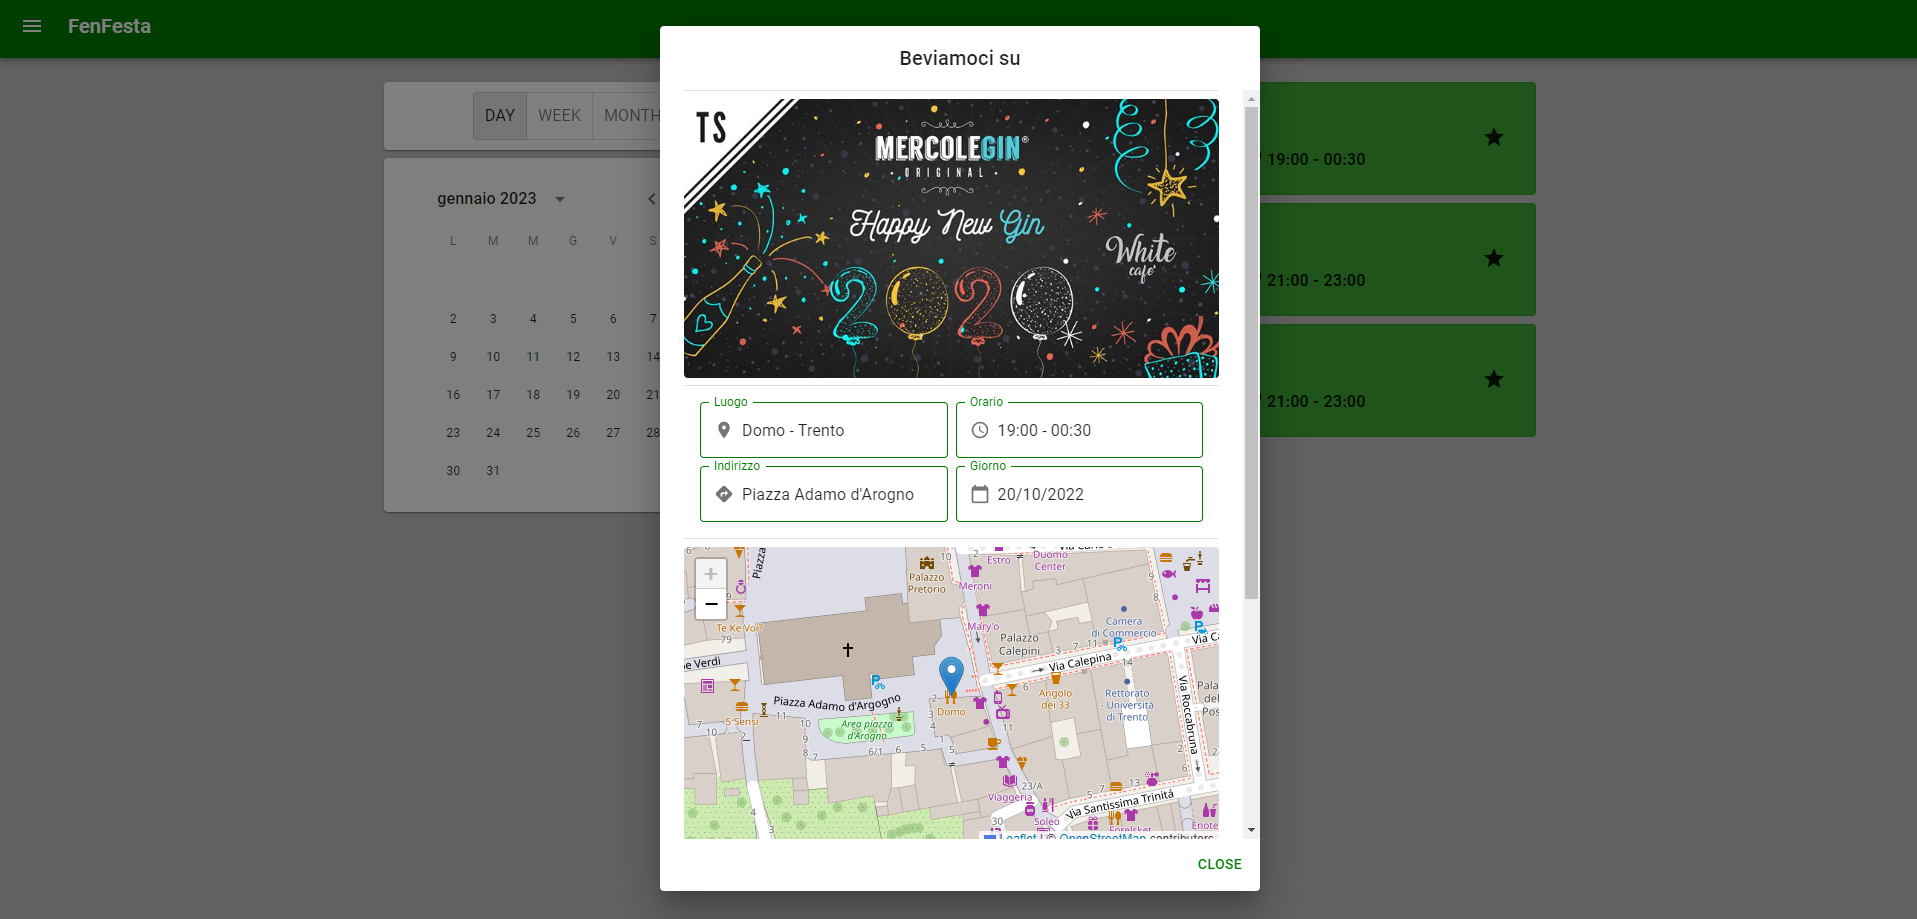
\includegraphics[scale=0.3]{Visualizza_Evento.png}
        \end{center}
    \item[] In questa sezione sono contenute tutte le informazioni relative all'evento (prese dal database). Sono presenti: immagine dell'evento, nome, data, orario, luogo, descrizione, tags, numero partecipanti, tasto “Partecipo”, tasto “Salva Evento”.
    \item[] Tramite il primo tasto viene aggiunta una persona al counter dei partecipanti; con la pressione del secondo, invece, si viene notificati della prossimità dell'evento tramite mail, il giorno stesso dell'evento.
    \item[] Questa schermata viene visualizzata sia quando si seleziona un evento dall'Elenco sia selezionando l'evento attraverso la Mappa
\end{description}
\subsection{Creazione Evento}
\begin{description}
    \item[] \begin{center}
            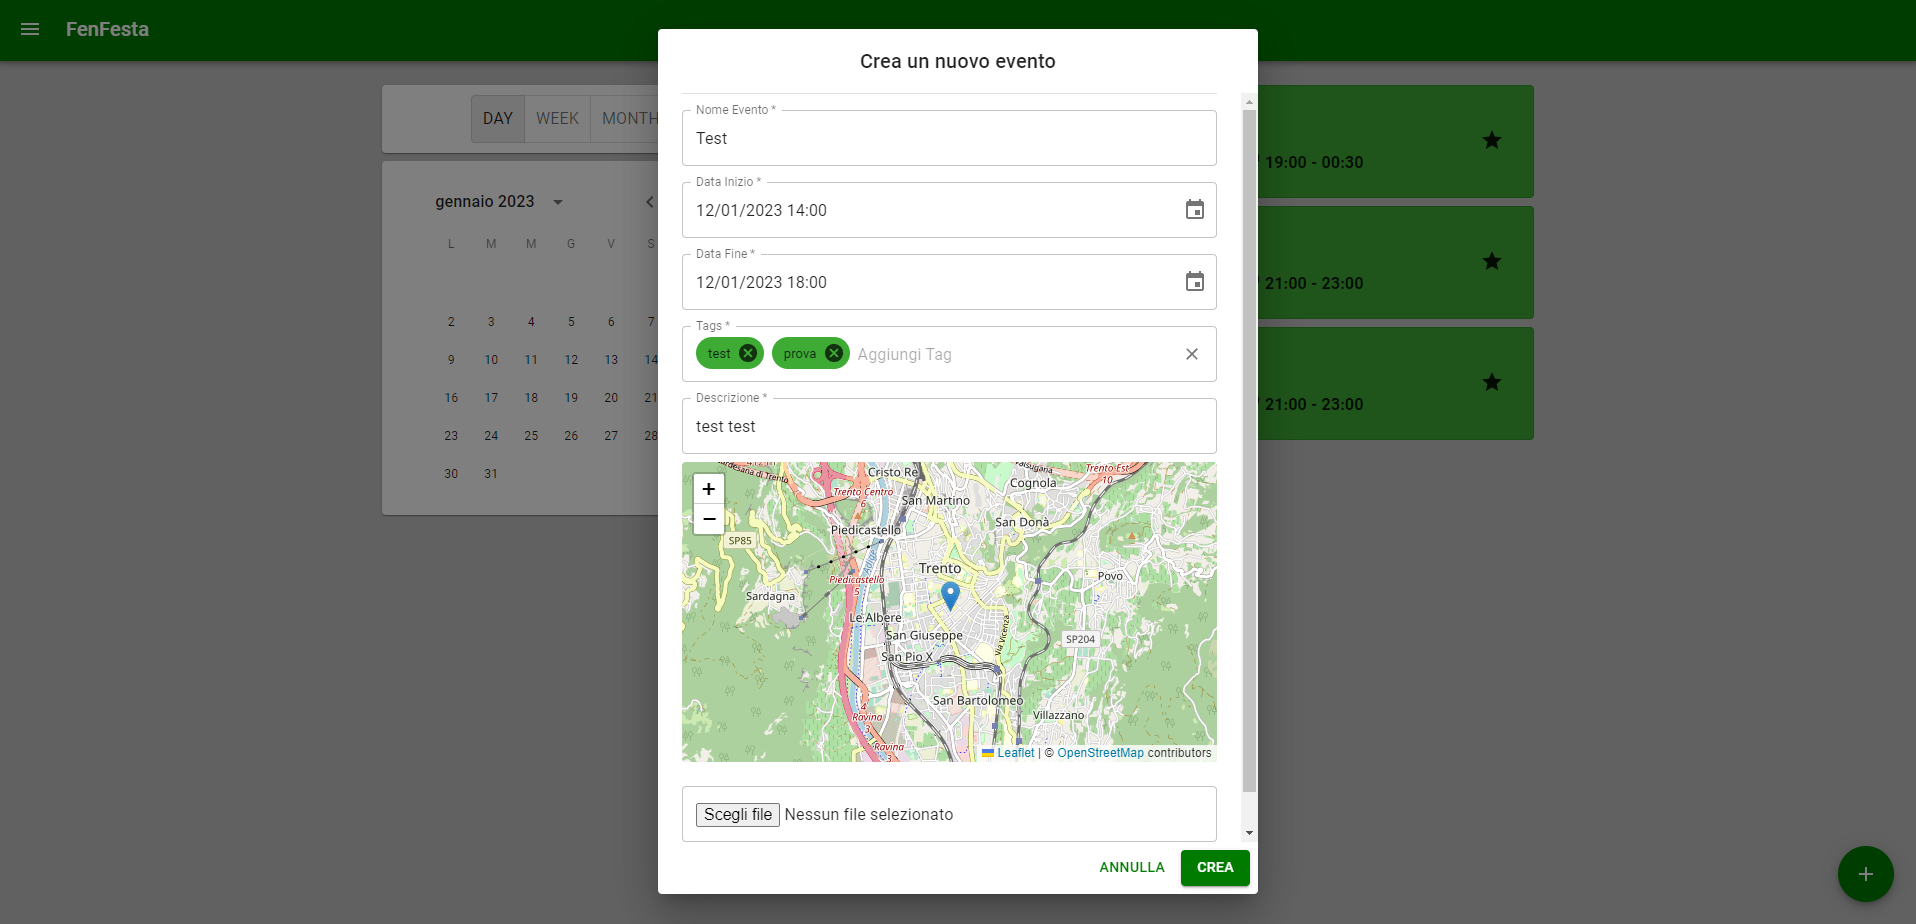
\includegraphics[scale=0.3]{Creazione_Evento.png}
        \end{center}
    \item[] Mediante la pressione di un tasto con l'icona di un + in una delle due schermate: Elenco o Mappa Eventi, e solo se si ha un account organizzatore, viene aperta la schermata di creazione Evento. È presente un form per l'inserimento di tutte le informazioni necessarie per la creazione, quali: immagine dell'evento, nome, data e orario, luogo, descrizione, tags.
    \item[] Premendo il tasto “Crea”, l'evento verrà registrato nel database e inserito nell'elenco eventi visualizzato tramite Mappa o Calendario
\end{description}
\clearpage
\section{GitHub Repository and Deployment Info}
\begin{description}
    \item[] Il progetto FenFesta è disponibile al seguente link: \url{https://github.com/T42CaCaGhi-Project}
    \item[] Per esegiure il front-end è necessario clonare la repository e successivamente utlizzare i comandi:
        \begin{enumerate}
            \item \texttt{npm install} per installare le varie dipendenze
            \item \texttt{npm start} per far partire il front-end
        \end{enumerate}
    \item[] Per esegiure il back-end è necessario clonare la repository e successivamente utlizzare i comandi:
        \begin{enumerate}
            \item \texttt{npm install} per installare le varie dipendenze
            \item \texttt{npm start} per far partire il back-end
        \end{enumerate}
    \item[] Per esegiure i test sulle API è necessario clonare la repository del back-end e successivamente utlizzare i comandi:
        \begin{enumerate}
            \item \texttt{npm install} per installare le varie dipendenze
            \item \texttt{npm run test} per far partire i test sulle API
        \end{enumerate}
\end{description}
\clearpage
\section{Testing}
\begin{description}
    \item[] Sono stati effettuati dei test usando jest su tutte le API implementate coprendo tutte o quasi (ad eccezione di errori interni del sistema) le tipologie di risposta identificate a partire dalle figure \hyperref[img:6]{6}, \hyperref[img:7]{7} e \hyperref[img:8]{8}.
    \item[] I test vengono eseguiti in modo sequenziale resettando e ripopolando dopo ogni test un database utilizzato esclusivamente per il testing.
    \item[] Il comando con cui vengono eseguiti i test è '\textbf{jest --runInBand --coverage}', è stato generata quindi anche la cartella \textbf{coverage} contenente il file \textbf{index.html} che se aperto in un browser fornisce informazioni addizionali sul completamento dei test effettuati.
    \item[] Tutti i test eseguiti sono riusciti. Nella seguente immagine è possibile vedere come il 100\% delle funzioni viene coperto e quasi sempre la copertura delle righe di codice supera il 90\% (principalmente vengono saltate porzioni di codice che gestiscono eventuali errori interni al sistema che non si sono verificati durante il testing).
    \item[] \begin{center}
            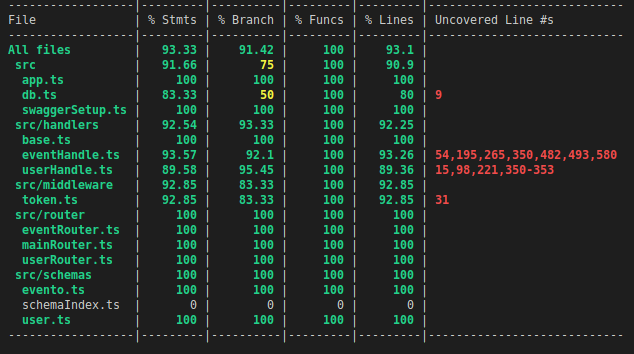
\includegraphics[scale=0.5]{testOut.png}
        \end{center}
        \clearpage
    \item[] Di seguito proponiamo un esempio dei test effettuati. La struttura dei test effettuati è la stessa per ogni test: i vari test sono raggruppati per API (salvo una singola eccezione dove era necessario un ambiente differente, per questo il test è stato svolto in maniera isolata) e divisi in due file, uno contenente i test per le API con percorso \textbf{/api/user} e uno contenentei test per le API con percorso \textbf{/api/event}.
    \item[] \begin{center}
            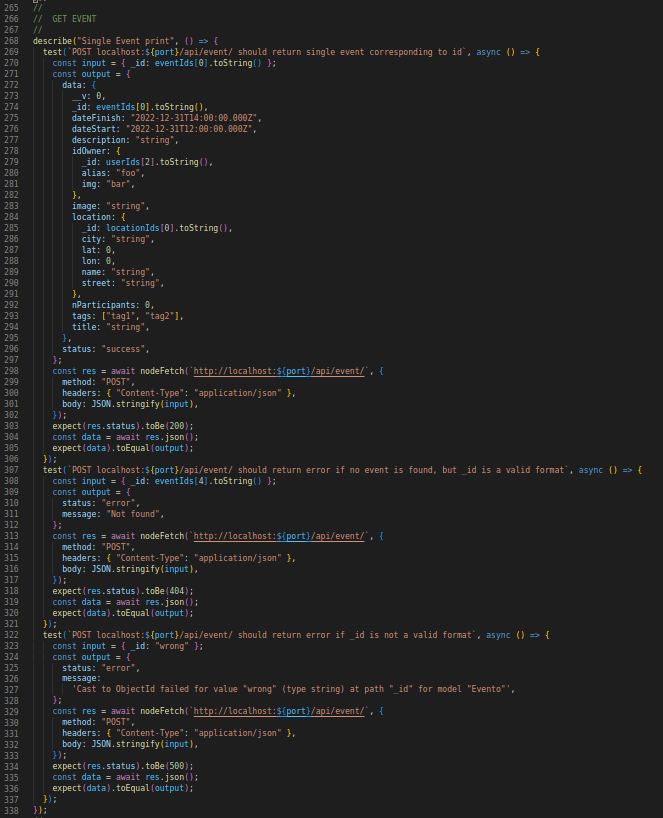
\includegraphics[scale=0.7]{getUserTest.png}
        \end{center}
\end{description}
\clearpage
\subsection{Testing API User}
\subsubsection{POST /api/user/new}
\begin{description}
    \item[] Ha successo se sia la password che la mail vengono fornite e se la mail è unica.
    \item[] Fallisce se uno dei due dati non viene fornito.
    \item[] Fallisce se la mail è già in uso.
\end{description}
\subsubsection{POST /api/user/login}
\begin{description}
    \item[] Ha successo se la mail e la password fornite identificano un utente creato in precedenza.
    \item[] Fallisce se le credenziali sono incomplete.
    \item[] Fallisce se la password non è corretta.
    \item[] Fallisce se la mail non identifica un utente precedentemente creato.
\end{description}
\subsubsection{POST /api/user/delete}
\begin{description}
    \item[] Ha successo se la mail e la password fornite identificano un utente creato in precedenza.
    \item[] Fallisce se il token non è corretto,
    \item[] Ha successo se chi richiede l'eliminazione di un utente che esiste è un admin.
    \item[] Fallisce se l'email non è corretta.
\end{description}
\subsubsection{POST /api/event/all}
\begin{description}
    \item[] Ha successo se esistono eventi nel database.
    \item[] Fallisce se non ci sono eventi nel database.
\end{description}
\subsubsection{POST /api/event/}
\begin{description}
    \item[] Ha successo se l'ID inserito è riferito ad un evento che esiste nel DB.
    \item[] Fallisce in caso contrario.
    \item[] Fallisce se l'ID fornito non è nel formato corretto di un ID di MongoDB.
\end{description}
\subsubsection{POST /api/event/new}
\begin{description}
    \item[] Ha successo se il request body è corretto e lo user è autorizzato.
    \item[] Fallisce se il request body è corretto ma lo user non è autorizzato.
    \item[] Fallisce se il request body è corretto, lo user è autorizzato, ma esiste già un evento con lo stesso titolo e la stessa data di inizio
\end{description}
\subsubsection{POST /api/event/modify}
\begin{description}
    \item[] Ha successo se se stiamo modificanto un evento che esiste nel DB e se lo user è autorizzato (organizzatore).
    \item[] Ha successo se se stiamo modificanto un evento che esiste nel DB e se lo user è autorizzato (admin).
    \item[] Fallisce se lo user non è autorizzato.
    \item[] Fallisce se si sta cercando di modificare un evento che non esiste.
\end{description}
\subsubsection{POST /api/event/delete}
\begin{description}
    \item[] Ha successo se l'evento esiste e lo user è autorizzato (orgganizzatore).
    \item[] Ha successo se l'evento esiste e lo user è autorizzato (admin).
    \item[] Fallisce se lo user non è autorizzato.
    \item[] Fallisce se l'evento non esiste.
\end{description}
\subsubsection{POST /api/event/tag}
\begin{description}
    \item[] Ha successo se almeno un evento contiene il/i tag presenti nel request body.
    \item[] Fallisce se nessun evento contiene i tag desiderati.
\end{description}
\subsubsection{POST /api/event/period}
\begin{description}
    \item[] Ha successo se esiste almeno un evento nel periodo scelto (sia esso giorno, settimana o mese).
    \item[] Fallisce se non viene trovato alcun evento.
\end{description}
\subsubsection{POST /api/event/preferito}
\begin{description}
    \item[] Ha successo se l'evento esiste e lo user si identifica correttamente con il suo token (aggiunta dell'evento ai preferiti).
    \item[] Ha successo se l'evento esiste e lo user si identifica correttamente con il suo token (rimozione dell'evento dai preferiti).
    \item[] Fallisce se il token non è valido.
    \item[] Fallisce se l'evento non esiste.
\end{description}
\end{document}